\documentclass[11pt,a4paper]{article}
% \documentclass[11pt]{amsart}
\usepackage[utf8]{inputenc}
\usepackage[margin=1in]{geometry}
\usepackage{color}
\usepackage{graphicx}
\usepackage{microtype}
\usepackage{array}
\usepackage{verbatim}
\usepackage{caption}
\usepackage{subcaption}
\usepackage{amsmath,amsthm,amsfonts,amssymb,latexsym}
\usepackage{bbm}
\usepackage{setspace}
\usepackage{xparse}
\usepackage{epstopdf}
\usepackage{pgf}
\usepackage[colorlinks=true,citecolor=blue]{hyperref}
\usepackage[nameinlink,capitalise]{cleveref}

\usepackage[style=trad-abbrv,doi=false,url=false,isbn=false,backend=biber]{biblatex}
\DeclareFieldFormat{volume}{volume \textbf{#1}}
\DeclareFieldFormat[article]{volume}{\textbf{#1}}
\addbibresource{main.bib}

\usepackage{tikz}
\usepackage{tikz-cd}
\usepackage{pgfplotstable}
\pgfplotsset{compat=1.14}
\usetikzlibrary{patterns}
\usetikzlibrary{calc}
\usetikzlibrary{angles}
\usetikzlibrary{quotes}
\usetikzlibrary{external}

\onehalfspacing
% \setlength{\parskip}{6pt}

\DeclareDocumentCommand\abs{s m} {\IfBooleanTF{#1}{\left|#2\right|}{\left|#2\right|}}
\DeclareDocumentCommand\cont{o m o} {C\IfNoValueF{#1}{^{#1}}(#2\IfNoValueF{#3}{;#3})}
\DeclareDocumentCommand\contc{o m o} {C_c\IfNoValueF{#1}{^{#1}}(#2\IfNoValueF{#3}{;#3})}
\DeclareDocumentCommand\sobolev{m m o} {H^{#1}(#2 \IfNoValueF{#3}{,#3})}
\DeclareDocumentCommand\lp{m m o} {L^{#1}\left(#2 \IfNoValueF{#3}{,#3}\right)}
\DeclareDocumentCommand\norm{s m o} {\IfBooleanTF{#1}{\|#2\|}{\left\|#2\right\|}\IfNoValueF{#3}{_{#3}}}
\DeclareDocumentCommand\seminorm{m o o} {\left|#1\right|\IfNoValueF{#2}{_{#2 \IfNoValueF{#3}{,#3}}}}
\DeclareDocumentCommand\ip{s m m o} {\IfBooleanTF{#1}{\langle #2,#3 \rangle}{\left\langle #2,#3 \right\rangle}\IfNoValueF{#4}{_{#4}}}
\DeclareDocumentCommand\dup{m m o} {\left\langle{#1,#2}\right\rangle\IfNoValueF{#3}{_{#3', #3}}}
\DeclareDocumentCommand\gaussian{O{0} O{I}} {g_{#1, #2}}
\DeclareDocumentCommand\littleo{s o m} {o\IfNoValueF{#2}{_{#2}}\IfBooleanTF{#1}{(#3)}{\left(#3\right)}}
\DeclareDocumentCommand\bigo{s o m} {\mathcal O\IfNoValueF{#2}{_{#2}}\IfBooleanTF{#1}{(#3)}{\left(#3\right)}}


\DeclareMathOperator*{\argmax}{arg\,max}
\DeclareMathOperator*{\argmin}{arg\,min}
\DeclareMathOperator*{\re}{Re}
\DeclareMathOperator*{\trace}{tr}
\DeclareMathOperator{\Span}{span}
\DeclareMathOperator{\sym}{sym}
\DeclareMathOperator{\sign}{sign}
\DeclareMathOperator{\diag}{diag}
\DeclareMathOperator{\id}{id}

% \DeclareMathOperator{\e}{e}
\newcommand{\e}{\mathrm{e}}

\newcommand{\revision}[1]{\textcolor{blue}{#1}}
\renewcommand{\revision}[1]{#1}
\newcommand{\gab}[1]{\textcolor{darkgreen}{#1}}
\newcommand{\commut}[2]{[#1, #2]}
\newcommand{\laplacian}{\Delta}
\newcommand{\correlation}[1]{\left< #1 \right>}
\newcommand{\dummy}{\,\cdot\,}
\newcommand{\expect}[0]{\mathbf{E}}
\newcommand{\proba}[0]{\mathbf{P}}
\newcommand{\var}[0]{\mathbf{V}}
\newcommand{\iip}[2]{\left(\!\left(#1, #2\right)\!\right)}
\newcommand{\nat}{\mathbf N}
\newcommand{\poly}{\mathbf P}
\newcommand{\real}{\mathbf R}
\newcommand{\integer}{\mathbf Z}
\newcommand{\torus}{\mathbf T}
\newcommand{\grad}{\nabla}
\newcommand{\hess}{\nabla^2}
\newcommand{\vect}[1]{\boldsymbol{\mathbf #1}}
\newcommand{\mat}[1]{\vect #1}
\renewcommand{\det}[1]{\mathrm{det} \left( #1 \right)}
\renewcommand{\d}{\mathrm d}
\renewcommand{\t}{\mathsf T}
% \renewcommand{\t}{t}

\makeatletter
\DeclareDocumentCommand \derivative{s m o m}{%
    \def\@der{\IfBooleanTF{#1}{\mathrm{d}}{\partial}}
    \def\@default{%
        \mathchoice{%
                \frac{%
                    \@der\ifnum\pdfstrcmp{#2}{1}=0\else^{#2}\fi {\IfNoValueTF{#3}{}{#3}}
                }{%
                    \@for\@token:={#4}\do{\@der \@token}
                }
            } {%
                \@for\@token:={#4}\do{\@der_\@token} \IfNoValueTF{#3}{}{#3}
            } {} {}
    }
    \IfBooleanTF{#1}{\IfNoValueTF{#3}{\@default}{%
                #3%
                \ifnum\pdfstrcmp{#2}{1}=0'\else%
                \ifnum\pdfstrcmp{#2}{2}=0''\else%
                \ifnum\pdfstrcmp{#2}{3}=0^{(3)}\else%
                \ifnum\pdfstrcmp{#2}{4}=0^{(4)}\else%
                \ifnum\pdfstrcmp{#2}{5}=0^{(5)}\else%
                ^{(#2)}\fi\fi\fi\fi\fi
            }
        }{\@default}
}
\makeatother

\definecolor{darkred}{rgb}{.5,0,0}
\definecolor{darkgreen}{rgb}{0,.5,0}
\definecolor{darkblue}{rgb}{0,0,.5}
\newcommand{\red}[1]{\textcolor{darkred}{#1}}
\newcommand{\green}[1]{\textcolor{darkgreen}{#1}}

\theoremstyle{plain}
\newtheorem{assumption}{Assumption}[section]
\newtheorem{lemma}{Lemma}[section]
\newtheorem{corollary}{Corollary}[section]
\newtheorem{theorem}{Theorem}[section]
\newtheorem{proposition}{Proposition}[section]
\newtheorem{result}{Result}[section]
\newtheorem{remark}{Remark}[section]
\newtheorem{example}{Example}[section]
\numberwithin{equation}{section}

\newcounter{urbainCounter}
\newcommand{\urbain}[1]{\stepcounter{urbainCounter}\red{\arabic{urbainCounter}.} \green{#1}}
\crefname{equation}{}{}
\crefname{paragraph}{\S\!}{\S}
% \crefname{figure}{Figure}{Figures}
% \crefname{section}{Section}{Sections}

\newcommand{\email}[1]{\href{#1}{#1}}
\newcommand{\orcidcolor}{ORC\textcolor{orcidlogocol}{ID}}
\newcommand{\orcid}[1]{\href{https://orcid.org/#1}{
\includegraphics[width=.4cm]{z_orcid.pdf}}}

%---------------- GABRIEL ------------
\usepackage{enumerate}
\newcommand{\eps}{\varepsilon}
\newcommand{\dps}{\displaystyle}
\newcommand{\cX}{\mathcal{X}}
\newcommand{\ri}{\mathrm{i}}
\renewcommand{\leq}{\leqslant}
\renewcommand{\geq}{\geqslant}
\renewcommand{\le}{\leqslant}
\renewcommand{\ge}{\geqslant}
% \usepackage{todonotes}
\usepackage{mathrsfs}

% BODY {{{1
\date{\today}
\title{Mobility estimation for Langevin dynamics using control variates}
\author{%
  % G.A. Pavliotis\thanks{Department of Mathematics, Imperial College London (\email{g.pavliotis@imperial.ac.uk})}%
  % \hspace{2mm}\orcid{0000-0002-3468-9227}%
  % \and G. Stoltz\thanks{CERMICS, \'Ecole des Ponts, France \& MATHERIALS, Inria Paris (\email{gabriel.stoltz@enpc.fr})}
  % \hspace{2mm}\orcid{0000-0002-2797-5938}%
  % \and U. Vaes\thanks{Department of Mathematics, Imperial College London (until October 2020) and MATHERIALS, Inria Paris (since November 2020) (\email{urbain.vaes@inria.fr})}%
  % \hspace{2mm}\orcid{0000-0002-7629-7184}%
}

\begin{document}
\maketitle

\begin{abstract}
    The scaling of the mobility of multi-dimensional Langevin dynamics in a periodic potential as the friction vanishes is not well understood for non-separable potentials.
    Theoretical results are lacking,
    and numerical calculation of the mobility in the underdamped regime is challenging because
    the computational cost is inversely proportional to the friction coefficient.
    In this note, we propose a new variance-reduction method based on control variates for efficiently estimating the mobility of Langevin-type dynamics.
    We provide bounds on the bias and variance of the proposed estimator,
    and we illustrate its efficacy through numerical experiments,
    first in simple one-dimensional settings
    and then for two-dimensional Langevin dynamics.
    Our results corroborate previous numerical evidence that
    the mobility scales as~$\gamma^{-\alpha}$ in the low friction regime for a simple non-separable potential.
\end{abstract}

\section{Introduction}%
Langevin dynamics model the evolution of a system of particles interacting with an environment at fixed temperature.
They are widely used for the calculation of macroscopic properties of matter in molecular simulation.
Assuming a diagonal mass matrix,
the standard Langevin dynamics, sometimes called underdamped Langevin dynamics,
reads after appropriate non-dimensionalization~\cite[Section 2.2.4]{MR2681239}
\begin{subequations}
\label{eq:langevin}
\begin{align}
    \label{eq:langevin_q}
    \d q_t &= p_t \, \d t, \\
    \label{eq:langevin_p}
    \d p_t &= - \grad V(q_t) \, \d t - \gamma \, p_t \, \d t + \sqrt{2 \gamma \beta^{-1}} \, \d \vect W_t.
\end{align}
\end{subequations}
Here $q_t \in \torus^d$ and $p_t \in \real^d$ are the position and velocity variables,
with~$\torus^d = \real^d / 2\pi \integer^d$ the $d$-dimensional torus with period $2 \pi$.
The parameter $\gamma$ is a dimensionless parameter we call the friction,
$V$ is periodic potential
and~$\vect W_t$ is a standard $d$-dimensional Brownian motion.
% $M$ is the mass matrix,
% For simplicity we assume that $M = m I_d$,
% where $I_d \in \real^{d \times d}$ is the identity matrix.
% In this case $(\widetilde q_t, \widetilde p_t) := (q_{\sqrt{m} t}, m^{-1/2} p_{\sqrt{m} t})$
% is a weak solution of~\eqref{eq:langevin} with $m = 1$ and $\gamma$ replaced by $\gamma/\sqrt{m}$,
% so to further simplify we assume $m = 1$,
% keeping in mind that asymptotic results for the case $m \neq 1$ can be deduced from this transformation;
% see~\cite[Section 2.2.4]{MR2681239} for a more detailed motivation of this simplification.
% keeping in mind that results obtained in the limit;
We recall that the dynamics~\eqref{eq:langevin} is ergodic with respect to the Boltzmann--Gibbs measure
\begin{equation}
    \label{eq:invariant_measure}
    \mu(\d q \, \d p) = \frac{1}{Z} \exp \bigl( - H(q, p)  \bigr) \, \d q \, \d p,
    \qquad H(q, p) = V(q) + \frac{\abs{p}^2}{2},
\end{equation}
with $Z$ the normalization constant.
It will be convenient to also introduce the marginal densities
\begin{equation}
    \label{eq:definition_prob_measures}
    \nu(\d q) = \frac{\e^{- \beta V(q)} \, \d q}{\int_{\torus^d}\e^{-\beta V(\widetilde q)} \d \widetilde q},
    \qquad \kappa(\d p) = \left( \frac{\beta}{2 \pi} \right)^{d/2}\exp \biggl( - \beta \frac{\abs*{p}^2}{2} \biggr) \d p.
\end{equation}

The mobility in direction $\vect e$ for dynamics~\eqref{eq:langevin} provides information on the behavior of the system
in response to an external forcing $\eta \vect e$ with magnitude~$\eta$ on the velocity process.
By analogy with macroscopic laws,
it is defined as the proportionality constant,
in the limit of a small forcing,
between the induced average velocity and the strength  of the forcing.
More precisely,
the mobility is defined mathematically as
\[
    D^{\gamma}_{\vect e} = \lim_{\eta \to 0} \frac{1}{\eta}\expect_{\mu_{\eta}} (\vect e^\t p),
\]
where $\mu_{\eta}$ is the invariant probability distribution of~\eqref{eq:langevin} when
an additional drift term $\eta \vect e$ is present on the right-hand side of~\eqref{eq:langevin_p}.
Except when $\eta = 0$ where we recover~\eqref{eq:invariant_measure},
the measure~$\mu_{\eta}$ is not known explicitly,
and so $D_{\vect e}^{\gamma}$ cannot be obtained simply by numerical integration of the observable $\vect e^\t p$ with respect to this measure.
It turns out that $D_{\vect e}^{\gamma}$ is a quadratic function of $\vect e$,
and we can define the symmetric mobility matrix $D^{\gamma}$ from the directional mobility
using the parallelogram identity:
\[
    4 \vect e_1^\t D^{\gamma} \vect e_2
    = (\vect e_1 + \vect e_2) ^\t D^{\gamma} (\vect e_1 + \vect e_2)
    - (\vect e_1 - \vect e_2) ^\t D^{\gamma} (\vect e_1 - \vect e_2)
    = D^{\gamma}_{\vect e_1 + \vect e_2} - D^{\gamma}_{\vect e_1 - \vect e_2}.
\]

It can be shown that the mobility coincides with the so-called effective diffusion coefficient associated with the equilibrium dynamics~\eqref{eq:langevin}:
the diffusively rescaled position process $(\varepsilon q_{t/\varepsilon^2})_{t\geq0}$ converges as $\varepsilon \to 0$,
weakly in the space of continuous functions over compact time intervals,
to a Brownian motion in $\real^d$ with prefactor $\sqrt{2 D^{\gamma}}$.
In particular, by the continuous mapping theorem,
\begin{equation}
    \label{eq:einsteins_formula}
    D^{\gamma}_{\vect e}
    =\lim_{\varepsilon \to 0} \frac{\expect\abs{\vect e^\t (\varepsilon q_{t/\varepsilon^2} - \varepsilon q_0)}^2}{2 t}
    =\lim_{t \to \infty} \frac{\expect \abs{\vect e^\t (q_t - q_0)}^2}{2t}.
\end{equation}
suggesting that the mobility can be calculated by
estimating the mean square displacement at a sufficiently large time of the equilibrium dynamics~\eqref{eq:langevin}
using Monte Carlo simulation,
which is one of the approaches taken in~\cite{MR2427108}.
Specifically, given a number $J$ of realizations of the dynamics~\eqref{eq:langevin} over a sufficiently long time interval $[0, T]$,
the mobility can be estimated as
\begin{equation}
    \label{eq:naive_estimator}
    \widehat D^{\gamma}_{\vect e}
    = \frac{1}{J} \sum_{j=1}^{J} \frac{\abs{\vect e^\t (q^{(j)}_T - q^{(j)}_0)}^2}{2T}.
\end{equation}
The variance reduction approach we propose in the next section aims at reducing the mean square error of estimators of this type.

The mobility (or effective diffusion coefficient)
is also related to the solution of a partial differential equation (PDE) involving the generator of the Markov semigroup associated with~\eqref{eq:langevin},
which is given by
\begin{equation}
    \label{eq:decomposition_generator}
    \mathcal L
    = p \cdot \grad_q - \grad V \cdot \grad_p + \gamma \left( - p \cdot \grad_p + \laplacian_p \right)
    =: \mathcal L_{\rm Ham} + \gamma \mathcal L_{FD}.
\end{equation}
Specifically, it is possible to  show~\cite{pavliotis2008multiscale,MR3509213} that $D^{\gamma}_{\vect e} = \ip{\phi_{\vect e}}{\vect e^\t p}$,
where $\ip{\dummy}{\dummy}$ denotes the inner product of $\lp{2}{\mu}$ and $\phi_{\vect e}$ denotes the solution in $\lp{2}{\mu}$,
unique up to an additive constant,
of the Poisson equation
\begin{equation}
    \label{eq:poisson_equation}
    - \mathcal L \phi_{\vect e} = \vect e^\t p.
\end{equation}

The behavior of Langevin dynamics~\eqref{eq:langevin} depends on the value of the friction parameter~$\gamma$,
The overdamped limit $\gamma \to \infty$ is well understood;
in this limit, the rescaled position process $\{q_{\gamma t}\}$
converges, uniformly for $t$ in compact subintervals of $[0, \infty)$ almost surely~\cite{MR0214150} and weakly~\cite{MR4054345},
to the solution of the overdamped Langevin equation
\begin{equation}
    \label{eq:overdamped_langevin}
    \d q_t = - \grad V(q_t) + \sqrt{2 \beta^{-1}} \, \d \vect W_t.
\end{equation}
It is also possible to prove that $\gamma D^{\gamma} = D^{\rm ovd} + \bigo{\gamma^{-2}}$ as $\gamma \to \infty$,
where~$D^{\rm ovd}$ is the effective diffusion coefficient of overdamped Langevin dynamics,
and to derive explicit expressions for the correction terms by asymptotic analysis~\cite{MR2394704}.
The diffusion coefficient in the overdamped limit is given by $D^{\rm ovd}_{\vect e} = \norm{\vect e + \grad \chi_{\vect e}}[\nu]^2$,
where $\chi$ is the solution in~$\lp{2}{\mu}$ of the Poisson equation
\[
    - \mathcal L_{\rm ovd} \chi_{\vect e} = \vect e^\t \grad(q), \qquad \mathcal L_{\rm ovd} = - \grad V \cdot \grad + \laplacian,
\]
with $\mathcal L_{\rm ovd}$ is the generator of the Markov semigroup associated with~\eqref{eq:overdamped_langevin}.
A reasoning similar to that in~\cite[Proposition 4.1]{MR2394704} in the one-dimensional setting shows that,
in fact, $D^{\rm ovd}_{\vect e}$ is an upper bound for $\gamma D^{\gamma}_{\vect e}$ for all $\gamma > 0$.

The underdamped limit is much more difficult to analyze,
especially in the multi-dimensional setting.
In spatial dimension one, it was shown in~\cite{MR2394704} that $\gamma D^{\gamma} \to D^{\rm und}$ as $\gamma \to \infty$ for some limit~$D^{\rm und}$
that is also a lower bound for $\gamma D^{\gamma}$ for all $\gamma > 0$.
It is also possible~\cite[Lemma 3.4]{MR2394704}, in this case,
to show that the solution to the Poisson equation,
multiplied by $\gamma$, converges in $\lp{2}{\mu}$ to a limit as $\gamma \to 0$,
which can be calculated explicitly in simple settings~\cite{MR2427108}.
Despite the existence of an asymptotic result,
calculating the mobility for small $\gamma$ is challenging;
the vanishing spectral gap of the generator $\mathcal L$ when $\gamma \to 0$ makes deterministic methods ill-conditioned
and Monte Carlo methods very slow to converge.

The aforementioned asymptotic result for the underdamped limit extends to the multi-dimensional setting only when the potential is separable,
that is when $V$ can be decomposed as $V(q) = \sum_i V_i(q_i)$,
but no theoretical results exist in the non-separable case,
which was explored mostly by means of numerical experiments.
Early numerical results in~\cite{chen1996surface} show that the effective diffusion coefficient scales as~$\gamma^{-1/2}$ in the underdamped regime for a particular case of a non-separable periodic potential.
Later, in~\cite{Braun02},
different authors note that this behavior as~$\gamma^{-1/2}$ is valid only when $\gamma \in [0.01, 0.1]$,
but not for smaller values of the damping coefficient.
They conclude from simulation results that the effective diffusion coefficient scales as~$\gamma^{-\sigma}$ with $0 \leq \sigma \leq 1/3$ in the underdamped regime,
and suggest that $\sigma$ could be zero for all non-separable potentials.
More recently, in his thesis~\cite{roussel_thesis},
Roussel calculated the mobility of Langevin dynamics  using a control variates approach for linear response.
His results demonstrate clearly that, for a wide range of friction coefficients in the interval $[10^{-3}, 1]$
and in the particular case of the potential
\begin{equation}
    \label{eq:potential_julien}
    V(q) = - \cos(q_1) - \cos(q_2) + \delta \exp \bigl(\sin(q_1 + q_2)\bigr),
\end{equation}
the mobility scales as $\gamma^{- \sigma}$,
with an exponent $\sigma \in [0, 1]$ that depends on the degree $\delta$ of non-separability of the potential.

In this note,
we propose a variance reduction methodology, also based on control variates,
for calculating the mobility of Langevin-type dynamics using Einstein's formula~\eqref{eq:einsteins_formula}.
The control variate is constructed from an approximate solution to the Poisson equation~\eqref{eq:poisson_equation}.
Our contributions are the following.
\begin{itemize}
    \item
        We derive bounds on the bias and variance of the proposed estimator for the simple case of one-dimensional Langevin dynamics,
        in terms of the error on the solution to the Poisson equation~\eqref{eq:poisson_equation}.
        Our estimates show, in particular, that the Langevin dynamics should be integrated up to a time scaling as $\max(\gamma, \gamma^{-1})$ in order to control the bias of the estimator.
    \item
        We examine the performance of the approach for two different approximate solutions to the Poisson equation:
        one is obtained through the Fourier/Hermite Galerkin method developed in~\cite{roussel2018spectral},
        and the other is calculated from the limiting solution of the Poisson equation in the underdamped limit;
        see~\cite{MR2427108}.
    \item
        We apply the proposed variance reduction approach to the estimation of mobility for two-dimensional Langevin dynamics in a non-separable periodic potential.
        To this end, we construct an approximation to the Poisson equation by tensorization of approximations obtained in one spatial dimension.
        We study numerically the performance of this approach,
        and we present numerical results corroborating the asymptotic behavior as $\gamma^{-\sigma}$ for $\sigma \in (0, 1]$ of the effective diffusion coefficient
        observed in~\cite{roussel_thesis}.
    \item
        Using the proposed variance reduction approach
        for calculating the diffusion coefficient of generalized Langevin dynamics in the underdamped regime,
        we provide numerical evidence supporting the asymptotic behavior of the effective diffusion coefficient conjectured in our previous work~\cite{GPGSUV21} using formal asymptotics.
\end{itemize}
The rest of the paper is organized as follows.
In~\cref{sec:method},
we present a control variate approach for improving the naive Monte Carlo estimator~\eqref{eq:naive_estimator},
and we obtain bounds on the bias and variance of the improved estimator in the particular case of Langevin dynamics~\eqref{eq:langevin}.
In~\cref{sec:application_to_one_dimensional_langevin_type_dynamics},
we employ the proposed approach for calculating the mobility of one-dimensional Langevin and generalized Langevin dynamics,
as proof of concept,
and we assess the performance of different control variates in terms of variance reduction.
In~\cref{sec:applications_2d},
we present numerical results for two-dimensional Langevin dynamics,
exhibiting a scaling as $\gamma^{-\sigma}$ of the mobility in the underdamped regime.
\Cref{sec:conclusions_and_perspectives_for_future_work} is reserved for conclusions and perspectives for future work,
and the appendices contain technical results employed in~\cref{sec:application_to_one_dimensional_langevin_type_dynamics}.



\section{Method and theoretical results}%
\label{sec:method}%

Throughout this section,
we focus on the Langevin dynamics~\eqref{eq:langevin} for simplicity,
but the approach we present can be applied to other Langevin-type dynamics.
A few of the results and arguments we present, however,
are tailored specifically for Langevin dynamics and would have to be modified for more other dynamics.
We also assume throughout the section that $\bigl((q_t, p_t)\bigr)_{t\geq 0}$ is a solution of~\eqref{eq:langevin} with statistically stationary initial condition~$(q_0, p_0) \sim \mu$.

Let us fix a direction $\vect e$ and denote again by $\phi_{\vect e}$ the solution to the Poisson equation~\eqref{eq:poisson_equation}.
Since the number of independent realizations in Monte Carlo estimators
appears only as a divisor in the variance,
we study estimators based on one realization only.
That is, instead of~\eqref{eq:naive_estimator} we take as point of comparison the naive estimator
\begin{equation}
    \label{eq:simple_estimator}
    u(T) = \frac{\abs{\vect e^\t (q_T - q_0)}^2}{2T},
\end{equation}

We motivate in this section that
the following estimator of $D_{\vect e}$ is better than $u(T)$ provided that $\psi_{\vect e}$ is a sufficiently good approximation of $\phi_{\vect e}$:
\begin{subequations}
\begin{equation}
    \label{eq:improved_estimator}
    v(T) = d_{\psi}+ \frac{1}{2T} \left( \abs{\vect e^\t(q_T - q_0)}^2 - \abs{\xi_T}^2\right),
\end{equation}
where $d_{\psi} := \gamma \beta^{-1} \int \abs{\grad_p \psi_{\vect e}}^2 \, \d \mu$ and
\begin{align}
    \label{eq:definition_control_variate}
    \xi_T = \psi_{\vect e}(q_T, p_T) - \psi_{\vect e}(q_0, p_0) - \sqrt{2 \gamma \beta^{-1}} \int_{0}^{T} \grad_p \psi_{\vect e}(q_t, p_t) \cdot \d \vect W_t.
\end{align}
\end{subequations}
Note that $v(T) = u(T)$ if $\psi_{\vect e} = 0$,
and that $v(T) = D_{\vect e}^{\gamma}$ if $\psi_{\vect e} = \phi_{\vect e}$ since by It\^o's formula
\begin{equation}
    \label{eq:ito_control_variate}
    \xi_T = \int_{0}^{T} \mathcal L \phi_{\vect e}(q_t, p_t) \, \d t = - \int_0^T \vect e^\t p_t \, \d t = \vect e^\t (q_0 - q_T)
\end{equation}
in this case, and $d_{\phi} = D_{\vect e}^{\gamma}$.
In addition, using It\^o's isometry we verify formally that $v(T)$ is asymptotically unbiased as~$T \to \infty$ regardless of the choice of $\psi_{\vect e}$:
\[
    \lim_{T \to \infty} \expect \bigl( v(T) \bigr)
    = d_{\psi} + \gamma \beta^{-1} \int \lvert \grad \phi_{\vect e} \rvert^2 \, \d \mu - \gamma \beta^{-1} \int \lvert \grad \psi_{\vect e} \rvert^2 \, \d \mu
    = \gamma \beta^{-1} \int \lvert \grad \phi_{\vect e} \rvert^2 \, \d \mu = D_{\vect e}^{\gamma}.
\]
\begin{remark}
    In view of~\eqref{eq:ito_control_variate}
    it would have been equivalent, in the case where $\psi_{\vect e}$ is smooth,
    to define
    \(
        \xi_T = \int_{0}^{T} \mathcal L \phi_{\vect e}(q_t, p_t) \, \d t
    \)
    from the beginning.
    However, the definition~\eqref{eq:definition_control_variate} makes sense even if $\psi_{\vect e}$ is differentiable only once,
    and is therefore more widely applicable.
    Our results in this section focus on the case where $\psi_{\vect e}$ is at least twice differentiable for simplicity,
    but in~\cref{sec:application_to_one_dimensional_langevin_type_dynamics} we will employ approximations $\psi_{\vect e}$ which are differentiable only once.
\end{remark}

We now obtain more precise results on the bias and variance of $u(T)$ and $v(T)$.

\subsection{Bias of the estimators}%
We begin by studying the bias of $u(T)$.
Since the initial conditions are assumed statistically stationary,~$(q_0, p_0) \sim \mu$,
it holds that
\begin{equation}
\label{eq:bias_without_control}
\begin{aligned}
    \expect \bigl(u(T)\bigr)
    &= \frac{1}{2T} \expect \left( \int_{0}^{T} \vect e^\t p_{t} \, \d t \int_{0}^{T} \vect e^\t p_s \, \d s \right)
    = \frac{1}{2t} \left( \int_{0}^{T} \int_{0}^{T} \expect (\vect e^\t p_t) (\vect e^\t p_s) \, \d s \, \d t \right) \\
    &= \frac{1}{2t} \left( \int_{0}^{T} \int_{0}^{T} \ip{\e^{\abs{t - s} \mathcal L}(\vect e^\t p)}{\vect e^\t p} \, \d s \, \d t \right)
    =  \int_{0}^{T} \ip{\e^{t \mathcal L} (\vect e^\t p)}{\vect e^\t p} \left(1 - \frac{t}{T}\right) \d t  \\
    &= \int_{0}^{\infty} \ip{\e^{t \mathcal L}(\vect e^\t p)}{\vect e^\t p}  \d t - \int_{0}^{T} \ip{\e^{t \mathcal L} (\vect e^\t p)}{\vect e^\t p} \min\left\{1, \frac{t}{T}\right\} \, \d t.
    % D_{\phi} - \int_{0}^{\infty} \min\left(1, \frac{s}{t}\right) C_{\phi}(s) \, \d s.
\end{aligned}
\end{equation}
The first term is the effective diffusion coefficient
and the second term is the bias.
As a first attempt towards bounding the latter term,
we use a general bound for the Markov semigroup associated with Langevin dynamics~\cite{roussel2018spectral}
stating that
\begin{equation}
    \label{eq:decay_semigroup_general}
    \forall \gamma > 0, \qquad \forall t \geq 0, \qquad
    \norm*{ \e^{s \mathcal L} }[\mathcal B \left(L^2_0\left(\mu\right) \right)] \leq M \exp \bigl(- \lambda s \min\{\gamma, \gamma^{-1}\} \bigr)
\end{equation}
for appropriate constants $M > 0$ and $\lambda > 0$.
An application of this bound gives
\[
    \ip{\e^{s \mathcal L}(\vect e^\t p)}{\vect e^\t p}
    \leq \norm*{\e^{s \mathcal L}(\vect e^\t p)} \norm*{\vect e^\t p}
    \leq M \beta^{-1} \exp\bigl(- \lambda s \min\{\gamma, \gamma^{-1}\}\bigr),
\]
which leads to the following estimate on the bias:
\begin{equation}
    \label{eq:bias}
    \abs{\expect_{\mu} u(T) - D_{\vect e}^{\gamma}}
    \leq \frac{M}{\beta T}\int_{0}^{\infty} \exp\bigl(- \lambda s \min\{\gamma, \gamma^{-1}\}\bigr) s \, \d s
    = \frac{M \max \{\gamma^2, \gamma^{-2}\}}{\beta \lambda^2 T}.
\end{equation}
Since the effective diffusion coefficient scales as $\gamma^1$ in both the underdamped ($\gamma \to 0$) and overdamped limits ($\gamma \to \infty$)~\cite{MR2394704,MR2427108},
this estimate suggests that the relative bias of the estimator scales as $\max\{\gamma^{-1}, \gamma^3\} T^{-1}$ and that,
consequently, the integration time should scale as $T \propto \max\{\gamma^{-1}, \gamma^3\}$ in order to meet a given threshold on the relative error.
It turns out that the estimate~\eqref{eq:bias} is in fact not optimal,
and it is sufficient to choose $T \propto \gamma$ in the overdamped limit.
We can derive a sharper estimate from the following result:
\begin{proposition}
    \label{proposition:semigroup_meanzero_observable}
    Let $\Pi_p: \lp{2}{\mu} \ni u \mapsto  u - \int u(q, p) \, \d \kappa(p)$ and $\Pi_p^\perp = \id - \Pi_p$.
    Assume that $f$ and $g$ are smooth functions in $\Pi_p^\perp \lp{2}{\mu}$
    such that $\partial_q f \in \lp{2}{\mu}$ and $\partial_q h \in \lp{2}{\mu}$.
    Then there exist constants $K$ and $\kappa$ independent of $\gamma$, $f$ and $h$ such that
    \begin{equation}
        \label{eq:optimal_decay_correlation}
        \forall \gamma \geq 1, \quad
        \forall t \geq 0, \qquad
        \abs{\ip{\e^{t \mathcal L}f}{h}}
        \leq K \norm{f}[1_q]  \norm{h}[1_q] \left( \gamma^{-2} \e^{- \kappa \gamma^{-1} t} + \e^{-\kappa  \gamma t} \right),
    \end{equation}
    where $\norm{\dummy}[1_q] = \norm{\dummy} + \norm{\grad_q \dummy}$.
\end{proposition}
Applying this result with $f(q, p) = h(q, p) = \vect e^\t p$, we obtain
\begin{equation*}
    \forall \gamma \geq 1, \qquad
    \abs{\expect_{\mu} u(T) - D}
    \leq \frac{K}{T}\int_{0}^{\infty} \left( \gamma^{-2} \e^{- \kappa \gamma^{-1} s} + \e^{-\kappa  \gamma s} \right)  s \, \d s
    \leq \frac{K}{\kappa T},
\end{equation*}
showing that the relative bias in fact scales as~$\max\{\gamma^{-1}, \gamma\} T^{-1}$,
and so it is sufficient to take $T \propto \gamma$ to control the bias in the overdamped limit.
Despite this improvement,
the computational cost of calculating the effective diffusion coefficient from Monte Carlo simulation in the overdamped regime is prohibitive,
because the time step must scale as $\gamma^{-1}$ in order to accurately integrate the Langevin dynamics,
leading to a computational cost in the overdamped limit scaling as $\gamma^2$.
The proof of \cref{proposition:semigroup_meanzero_observable} is postponed to \cref{sec:auxiliary_technical_results}.
In this section,
we motivate the result by scrutinizing two settings where
explicit expressions of the bias, or of the velocity auto-correlation,
can be obtained:
constant potential and quadratic potential.
\begin{example}
    [Constant potential]
    \label{example:constant}
    Consider the case where $V(q) = 0$ in one dimension.
    In this case, the solution to the Poisson equation $- \mathcal L \phi = p$ is given by $\phi(q, p) = \gamma^{-1} p$,
    and applying Itô's formula to this function we obtain
    (note that this also follows directly from~\eqref{eq:langevin_p})
    \[
        \gamma^{-1}(p_t - p_0) = - \int_{0}^{t} p_s \, \d s + \sqrt{2 \gamma^{-1} \beta^{-1}} (W_t - W_0)
        = q_0 - q_t + \sqrt{2 \gamma^{-1} \beta^{-1}} W_t.
    \]
    Using the explicit solution to the Ornstein--Uhlenbeck equation satisfied by $p$,
    we deduce that
    \begin{align*}
        q_t - q_0
        &= - \gamma^{-1} \left( p_0 \left(\e^{-\gamma t} - 1\right) + \sqrt{2 \gamma \beta^{-1}}\int_{0}^{t} \e^{-\gamma (t - s)} \, \d W_s \right)
        + \sqrt{2 \gamma^{-1} \beta^{-1}} W_t \\
        &=  - \gamma^{-1} p_0 \left(\e^{-\gamma t} - 1\right) + \sqrt{2 \gamma^{-1} \beta^{-1}}\int_{0}^{t} \left(1 - \e^{-\gamma (t - s)}\right) \, \d W_s.
    \end{align*}
    Assuming $p_0 \sim \mathcal N(0, \beta^{-1})$,
    the right-hand side of this equation is a mean-zero Gaussian random variable and,
    using It\^o's isometry, we calculate that
    \[
        \expect \bigl( u(T) \bigr) = \frac{\expect \abs{q_T - q_0}^2}{2T} = \gamma^{-1} \beta^{-1} \left( 1 + \frac{1}{T \gamma} \left(\e^{-\gamma T} - 1\right) \right).
    \]
    In this example, the relative bias is bounded from above by $(T \gamma)^{-1}$.
    Furthermore,
    since $\frac{\lvert q_T- q_0 \rvert^2}{2T\sigma^2}$ is distributed according to $\chi^2(1)$,
    the variance of $u(T)$ is equal to
    \[
        \var \bigl(u(T)\bigr) = 2  \bigl(\expect u(T)\bigr)^2
        \xrightarrow[T \to \infty]{} 2 \lvert D^{\gamma} \rvert^2.
    \]
\end{example}

\begin{example}
    [Quadratic potential]
    \label{example:quadratic}
    Consider now the case of the quadratic confining potential $V(q) = \frac{k q^2}{2}$.
    In this case, the eigenfunctions of $\mathcal L$ are polynomials,
    with the linear ones and associated eigenvalues being
    \[
        v_{\pm}(q, p) =
        \left( \frac{\gamma \pm \sqrt{\gamma^2 - 4k}}{2} \right) q + p, \\
        \qquad
        \lambda_{\pm} = \frac{- \gamma \pm \sqrt{\gamma^2 - 4k}}{2}.
    \]
    The function $(q, p) \mapsto p$ is the following linear combination of these eigenfunctions:
    \[
        p =
        \left( \frac{-\gamma + \sqrt{\gamma^2 - 4k}}{2 \sqrt{\gamma^2 - 4k}} \right) v_+
        + \left( \frac{\gamma + \sqrt{\gamma^2 - 4k}}{2 \sqrt{\gamma^2 - 4k}} \right) v_-.
    \]
    Therefore, given that $\ip{v_+}{p} = \ip{v_-}{p} = \beta^{-1}$,
    the velocity autocorrelation function is
    \[
        \ip{\e^{t \mathcal L}p}{p} =
        \left( \frac{-\gamma + \sqrt{\gamma^2 - 4k}}{2 \beta \sqrt{\gamma^2 - 4k}} \right) \e^{\lambda_+ t} +
        \left( \frac{\gamma + \sqrt{\gamma^2 - 4k}}{2 \beta \sqrt{\gamma^2 - 4k}} \right) \e^{\lambda_- t} = T_1(t) + T_2(t).
    \]
    This function has a form consistent with the bound in \cref{proposition:semigroup_meanzero_observable},
    in that the factor multiplying the first term scales as $\bigo{\gamma^{-2}}$
    and $\lambda_+$ scales as $\bigo {\gamma^{-1}}$ as $\gamma \to \infty$.
    Note that, in this non-periodic case, the effective diffusion coefficient is equal to zero.
    % it holds that $\int_{0}^{\infty} T_1(t) \, \d t = \bigo{\gamma^{-1}}$
    % because the factor multiplying the exponential scales as $\bigo {\gamma^{-2}}$.
\end{example}

We now obtain a bound on the bias of the improved estimator $v(T)$.
\begin{proposition}
    [Bias of the estimator]
    Assume that $\mathcal L \psi_{\vect e} \in \lp{2}{\mu}$.
    \begin{itemize}
        \item \textbf{General bound for $\gamma \in (0, \infty)$:}
            With the same notation as in~\eqref{eq:bias},
            it holds that
            \begin{align}
                \label{eq:basic_bound_bias}
                \abs{\expect \bigl( v(T) \bigr) - D^{\gamma}_{\vect e}}
                \leq & \left( \frac{M \max\{\gamma^2, \gamma^{-2}\}}{T \lambda^2 } \right) \,  \norm{\vect e^\t p + \mathcal L \psi_{\vect e}}  \left(\beta^{-1/2} + \norm{\mathcal L \psi_{\vect e}} \right).
            \end{align}
        \item \textbf{Refined bound in the overdamped regime:}
        If also $\mathcal L \psi_{\vect e} \in \lp{2}{\mu}$ and $\grad_q \mathcal L \psi_{\vect e} \in \lp{2}{\mu}$,
        then there exists $C$ independent of $\gamma$, $T$ and $\psi_{\vect e}$ such that
        \begin{align}
            \notag
            \forall \gamma \geq 1, \qquad
            \abs{\expect \bigl( v(T) \bigr) - D_{\vect e}^{\gamma}}
            &\leq C T^{-1}
            \norm*{\vect e^\t p +  \mathcal L \psi_{\vect e}}[1_q] \, \bigl(1 + \norm{\mathcal L \psi_{\vect e}}[1_q] \bigr) \\
            \label{eq:refined_bound}
            &\quad + C T^{-1} \gamma^2 \norm{\Pi_p \mathcal L \psi_{\vect e}} \norm{\mathcal L \psi_{\vect e}}
        \end{align}
    \end{itemize}
\end{proposition}
\begin{remark}
    The right-hand side of~\eqref{eq:basic_bound_bias} is small when $\psi_{\vect e} \approx \phi_{\vect e}$,
    and when $\psi_{\vect e} = 0$ we recover the bound~\eqref{eq:bias} derived previously.
\end{remark}
\begin{proof}
Using Itô's formula for $\psi_{\vect e}$,
we have
\[
    \psi_{\vect e}(q_T, p_T) - \psi_{\vect e}(q_0, p_0)
    = \int_{0}^{T} (\mathcal L \psi_{\vect e}) (q_t, p_t) \, \d t + \sqrt{2 \gamma \beta^{-1}} \int_{0}^{T} \grad_p \psi_{\vect e} (q_t, p_t) \cdot \d W_t,
\]
and employing the same reasoning as in~\eqref{eq:bias_without_control} we obtain
\begin{align*}
    \expect_{\mu} v(T)
    &= d_{\psi} + \left( \frac{1}{2T} \right) \expect_{\mu} \biggl( \abs{\vect e^\t (q_T - q_0)}^2 - \biggl| \int_0^T {\mathcal L \psi}(q_t, p_t) \, \d t \biggr|^2 \biggr) \\
    &= d_{\psi} +  \frac{1}{2T}  \int_{0}^{T} \Bigl( \ip{\e^{t \mathcal L}(\vect e^\t p)}{\vect e^\t p} - \ip{\e^{t \mathcal L} \mathcal L \psi_{\vect e}}{\mathcal L \psi_{\vect e}} \Bigr) \min\left\{1, \frac{t}{T}\right\} \d t \\
    &= d_{\phi} - \int_{0}^{\infty} \min\left\{1, \frac{t}{T}\right\} \Bigl( \ip{\e^{t \mathcal L}(\vect e^\t p)}{\vect e^\t  p} - \ip{\e^{t \mathcal L} \mathcal L \psi_{\vect e}}{\mathcal L \psi_{\vect e}} \Bigr) \, \d t.
\end{align*}
In order to obtain~\eqref{eq:basic_bound_bias}, we write
\begin{align*}
    \ip{\e^{t \mathcal L}(\vect e^\t p)}{\vect e^\t p} - \ip{\e^{t \mathcal L} \mathcal L \psi_{\vect e}}{\mathcal L \psi_{\vect e}}
    &= \ip{\vect e^\t p + \mathcal L \psi_{\vect e}}{\e^{t \mathcal L} (\vect e^\t p) - \e^{t \mathcal L^*} \mathcal  L\psi_{\vect e}} \\
    &\leq \norm*{\vect e^\t p + \mathcal L \psi_{\vect e}}
    \left( \norm*{\e^{t \mathcal L}}[\mathcal B\left(L^2_0(\mu) \right)] \, \norm*{\vect e^\t p} + \norm*{\e^{t \mathcal L^*}}[\mathcal B\left(L^2_0(\mu) \right)] \norm{\mathcal L \psi_{\vect e}} \right) \\
    &\leq M \e^{- \lambda \min\{\gamma, \gamma^{-1}\} t} \norm*{\vect e^\t p + \mathcal L\psi_{\vect e}}  \left(\beta^{-1/2} + \norm{\mathcal L \psi_{\vect e}} \right),
\end{align*}
where the first inequality is justified in view of the fact that $\e^{t \mathcal L^*}$ and $\e^{t \mathcal L}$ have the same norm,
since the operator $\mathcal L^*$, which is the formal $\lp{2}{\mu}$ adjoint of $\mathcal L$,
coincides with $\mathcal L$ up to the sign of the Hamiltonian part.
We then obtain~\eqref{eq:basic_bound_bias} by employing the reasoning that led to~\eqref{eq:bias}.

To obtain the refined bound in the overdamped limit,
we write
\begin{align*}
    &\ip{\e^{t \mathcal L}(\vect e^\t p)}{\vect e^\t p)} - \ip{\e^{t \mathcal L} \mathcal L \psi_{\vect e}}{\mathcal L \psi_{\vect e}}
      = \ip{\e^{t \mathcal L} (\vect e^\t p)}{\vect e^\t p + (\id - \Pi_p) \mathcal L \psi_{\vect e}} \\
      &\qquad - \ip{\e^{t \mathcal L} \bigl(\vect e^\t p + (\id - \Pi_p) \mathcal L \psi_{\vect e}\bigr)}{(\id - \Pi_p) \mathcal L \psi_{\vect e}}
      - \ip{\e^{t \mathcal L} (\id - \Pi_p) \mathcal L \psi_{\vect e}}{\Pi_p \mathcal L \psi_{\vect e}}
    - \ip{\e^{t \mathcal L} \Pi_p \mathcal L \psi_{\vect e}}{\mathcal L \psi_{\vect e}}.
\end{align*}
The last two terms are bounded using the general bound on the Langevin semigroup~\eqref{eq:decay_semigroup_general},
\[
    \abs{\ip{\e^{t \mathcal L} (\id - \Pi_p) \mathcal L \psi_{\vect e}}{\Pi_p \mathcal L \psi_{\vect e}}}
    \vee \abs{\ip{\e^{t \mathcal L} \Pi_p \mathcal L \psi_{\vect e}}{\mathcal L \psi_{\vect e}}}
    \leq M \exp \left( - \lambda \min\{\gamma, \gamma^{-1}\} t\right) \norm{\Pi_p \mathcal L \psi_{\vect e}} \norm{\mathcal L \psi_{\vect e}},
\]
and the first two terms are bounded using \cref{proposition:semigroup_meanzero_observable}:
\begin{align*}
    \abs{\ip{\e^{t \mathcal L} (\vect e^\t p)}{\vect e^\t p + (\id - \Pi_p) \mathcal L \psi_{\vect e}}}
    &\leq C \norm*{\vect e^\t p + \mathcal L \psi_{\vect e}}[1_q] \, \zeta(t), \\
    \abs{\ip{\e^{t \mathcal L} \bigl(\vect e^\t p + (\id - \Pi_p) \mathcal L \psi_{\vect e}\bigr)}{(\id - \Pi_p) \mathcal L \psi_{\vect e}}}
    &\leq C \norm*{\vect e^\t p + \mathcal L \psi_{\vect e}}[1_q] \, \norm*{\mathcal L \psi_{\vect e}}[1_q] \, \zeta(t),
\end{align*}
where $\zeta(t) = \gamma^{-2} \e^{- \kappa \gamma^{-1} t } + \e^{- \kappa \gamma t}$.
Here we employed the fact that, for any $f \in \lp{2}{\mu}$ such that $\grad_q f \in \lp{2}{\mu}$,
it holds
\[
    \ip{\grad_q (\id - \Pi_p) f}{\grad_q \Pi_p f} = 0,
\]
and so $\norm{(\id - \Pi_p) f}[1_q] \leq \norm{\grad_q f}[1_q]$.
The bound~\eqref{eq:refined_bound} is then obtained using the same reasoning as that which gave~\eqref{eq:bias}.
\end{proof}

% \begin{remark}
%     In one spatial dimension, it is possible to modify a control variate $\psi$ in such a way that $\Pi_p \mathcal L \psi = 0$.
%     Let $\alpha^{\psi}_1(q) = \int \psi(q,p) \, \sqrt{\beta} p \, \d \kappa(p)$ and define
%     \[
%         \widetilde \psi = \psi(q,p) - \sqrt{\beta} p \left(  \alpha_1^{\psi}(q) - k \e^{\beta V(q)}   \right),
%         \qquad k = \frac{\int \alpha_1^{\psi}\!(q) \, \e^{\beta V(q)} \, \d \nu(q)}{\int \e^{2 \beta V(q)} \, \d \nu(q)}.
%     \]
%     Note that $\widetilde \psi$ is the $L^2(\mu)$ orthogonal projection of $\psi$ on the subspace of functions of the form
%     \[
%         f = \alpha_0(q) + \alpha_1 \, \e^{\beta V(q)} \, \sqrt{\beta} p + \alpha_2(q) \, H_2(p) + \alpha_3(q) H_3(p), \dotsc
%     \]
%     where $(H_i)_{i \geq 0}$ are appropriately rescaled Hermite polynomials.
%     The exact solution $\phi$ is of this form since $\Pi_p \mathcal L = \Pi_p \mathcal L_{\rm Ham} =  \Pi_p \partial_p \partial_q^*$,
%     and the kernel of $\partial_q^*$ is spanned by $\e^{\beta V(q)}$.
%     We can bound
%     \begin{align*}
%         \norm*{\widetilde \psi - \phi}[3]
%         &\leq  \norm{\psi - \phi}[3] + \norm{\widetilde \psi - \psi}[3] \\
%         & \norm{\psi - \phi}[3] \lvert \alpha_1^{\phi} - k \rvert \norm*{\e^{\beta V(q)}} \\
%         &= \norm{\psi - \phi} + \lvert \alpha_1^{\phi} - k \rvert \norm*{\e^{\beta V(q)}}.
%     \end{align*}
%     \begin{align*}
%         \Pi_p \partial_p \partial_q^* \widetilde \psi
%         &= \int \partial_p \partial_q^* \psi(q, \widetilde p) \, \d \kappa(\widetilde p)
%         -  \left(\partial_q^*\psi_1(q) +  k \left( \partial_q^* \e^{\beta V(q)} \right) \right)
%         = \partial_q^*\psi_1(q) - \partial_q^*\psi_1(q) - 0 = 0,
%     \end{align*}
%     and it is simple to check that our choice of $k$ guarantees that $\widetilde \psi = \psi$
%     if $\psi = \phi$ is the exact solution to the Poisson equation~\eqref{eq:poisson_equation}.
%     Notice that
%     \[
%         \widetilde \psi_{\vect e} - \phi_{\vect e} = \
%     \]
% \end{remark}

\subsection{Variance of the estimators}%
We now obtain bounds on the variance of the estimators $u(T)$ and $v(T)$.
It is difficult to obtain bounds that scale well both as $\gamma \to 0$ and $\gamma \to \infty$,
so here we aim to obtain bounds with a good scaling in the underdamped regime only,
as this is the interesting regime for the mobility.

\begin{proposition}
    There exists $C$ independent of $\gamma$, $T$ and $\psi_{\vect e}$ such that
    \begin{equation}
        \label{eq:variance_estimator}
        \var \bigl(v(T)\bigr)
        \leq
        C \left( T^{-1} \norm{\phi - \psi}[4]^2  + \gamma \norm{\grad_p \phi - \grad_p \psi}[4]^2 \right)
        \left( T^{-1} \norm{\phi + \psi}[4]^2  + \gamma \norm{\grad_p \phi + \grad_p \psi}[4]^2 \right),
    \end{equation}
    provided that all the terms on the right-hand side are finite.
\end{proposition}
\begin{remark}
    Note that the variance does not converge to zero in the limit as $T \to \infty$.
    The asymptotic behavior of the variance,
    which is in contrast with the usual behavior for estimators based on linear response,
    is made more precise in \cref{proposition:asymptotic_variance} below.
\end{remark}
\begin{remark}
    In order to assess the quality of estimator~\eqref{eq:variance_estimator} in the underdamped limit,
    let us consider the particular setting where $\psi_{\vect e} = 0$ in one dimension.
    In~\cite[Remark 6.10]{MR2394704},
    the authors prove that $\norm{\phi}[\lp{p}{\mu}] = \bigo{\gamma^{-1}}$ as $\gamma \to 0$ for every $p \in [1, \infty)$,
    and they conjecture that also $\norm{\partial_p \phi}[\lp{p}{\mu}] = \mathcal O(\gamma^{-1})$ in the same limit.
    Assuming this is true, the estimate~\eqref{eq:variance_estimator} gives
    \begin{equation}
        \label{eq:variance_scaling}
        \forall 0 < \gamma \leq 1, \qquad
        \var \bigl(v(T)\bigr)
        \leq C \left( T^{-1} \gamma^{-2} + \gamma^{-1} \right)^2.
    \end{equation}
    For an integration time $T$ scaling $\gamma^{-1}$,
    which is required in order to control the bias,
    we find that the variance scales as $\gamma^{-2}$,
    hence the relative standard deviation scales as $\mathcal O(1)$.
    In practice, this means that we can keep the number of Monte Carlo replicas constant as $\gamma \to 0$.
\end{remark}
\begin{proof}
    The proof is based on the crude inequality
    \begin{align}
        \notag
        \var \bigl(v(T)\bigr)
        &\leq \expect \left( \abs{v(T) - d_{\psi}}^2 \right)
        = \frac{1}{4 T^2} \expect \big( |q_T - q_0 - \xi_T|^2 |q_T - q_0 + \xi_T|^2 \big) \\
        \label{eq:bound_variance_two_factors}
        &\leq \frac{1}{4 T^2}
        {\Bigl(\expect \left(  |q_T - q_0 - \xi_T|^{2p} \right)\Bigr)^{\frac{1}{p}}} \,
        {\Bigl(\expect \left( |q_T - q_0 + \xi_T|^{2q} \right)\Bigr)^{\frac{1}{q}}},
        \qquad \frac{1}{p} + \frac{1}{q} = 1.
    \end{align}
    We recall that, by It\^o's formula, it holds
    \begin{align*}
        \phi_{\vect e}(q_T, p_T) - \phi_{\vect e}(q_0, p_0)
        &= - \int_{0}^{T} \, (\vect e^\t p_t) \, \d t + \sqrt{2 \gamma \beta^{-1}} \int_{0}^{T} \, \grad_p \phi_{\vect e} (q_t, p_t) \cdot \d \vect W_t, \\
        \psi_{\vect e}(q_T, p_T) - \psi_{\vect e}(q_0, p_0)
        &= \int_{0}^{T} \, \mathcal L \psi_{\vect e}(q_t, p_t) \, \d t + \sqrt{2 \gamma \beta^{-1}} \int_{0}^{T} \, \grad_p \psi_{\vect e} (q_t, p_t) \cdot \d \vect W_t.
    \end{align*}
    Denoting the It\^o integrals in these equations by $I_{\phi}$ and $I_{\psi}$ respectively,
    and using the short-hand notation $\chi_{s} = \chi_{\vect e}(q_s, p_s)$ for $\chi \in \{\phi, \psi\}$,
    we now bound
    \begin{align*}
        \expect \left( |q_T - q_0 + \xi_T|^{2p} \right)
        &= \expect \left( \abs{\phi_{0} - \phi_{T} - \psi_{0} + \psi_{T}  + I_{\phi} - I_{\psi}}^{2p} \right) \\
        &\leq 3^{2p-1} \left( \expect \left( \abs{\phi_t - \psi_t}^{2p} \right) + \expect \left( \abs{\phi_0 - \psi_0}^{2p} \right) + \expect \left( \abs{I_{\psi} - I_{\phi}}^{2p} \right) \right).
    \end{align*}
    The first two terms are bounded by $\norm{\phi_{\vect e} - \psi_{\vect e}}_{L^{2p}(\mu)}^{2p}$.
    Using a moment inequality for It\^o integrals~\cite[Theorem 7.1]{MR2380366}
    and the assumption of statistically stationary initial conditions,
    we can bound the last term as
    \begin{align*}
        \expect \left( \abs{I_{\psi} - I_{\phi}}^{2p} \right)
        &\leq \bigl(p(2p - 1)\bigr)^p \, \left(2 \gamma \beta^{-1}\right)^p \,  T^{p-1} \,
        \expect \int_{0}^{t} \abs{\grad_p \phi(q_s, p_s) - \grad_p \psi(q_s, p_s)}^{2p} \, \d s \\
        &= \bigl(p(2p - 1)\bigr)^p \, \left(2 \gamma \beta^{-1}\right)^p \,  T^{p} \, \int \abs{\grad_p \phi - \grad_p \psi}^{2p} \d \mu.
    \end{align*}
    Likewise, the second factor in~\eqref{eq:bound_variance_two_factors} can be bounded as
    \begin{align*}
        \expect \left( |q_T - q_0 - \xi_T|^{2q} \right)
        &\leq 3^{2q-1} \Bigl( 2 \norm{\phi_{\vect e} + \psi_{\vect e}}[L^{2q}(\mu)]^{2q} \\
        & \qquad + \bigl(q(2q - 1)\bigr)^q \, \left(2 \gamma \beta^{-1}\right)^q \, T^{q} \norm{\grad_p \phi_{\vect e} + \grad_p \psi_{\vect e}}[L^{4}(\mu)]^4 \Bigr).
    \end{align*}
    The statement is then obtained by letting $p = 2$.
\end{proof}

We now quantify more precisely the asymptotic variance of $v(T)$ as $T \to \infty$.
\begin{proposition}
    [Asymptotic variance]
    \label{proposition:asymptotic_variance}
    It holds that
    \begin{equation}
        \label{eq:asymptotic_variance}
        \var\bigl(v(T)\bigr) \xrightarrow[T \to \infty]{}
        2 d_{\phi}^2 + 2 d_{\psi}^2 - 4 \gamma^2 \beta^{-2} \left( \int \grad_p \phi_{\vect e} \cdot \grad_p \psi_{\vect e} \, \d \mu \right)^2.
    \end{equation}
    In particular, there exists a constant $C$ independent of $\gamma$ and $\psi_{\vect e}$ such that
    \begin{align}
        \label{eq:bounds_asymptotic_variance}
        2(d_{\phi} - d_{\psi})^2
        \leq \lim_{T \to \infty} \var \bigl(v(T)\bigr)
        \leq 2 (d_{\psi}^2 - d_{\phi}^2) + C \max\{\gamma^{1/2}, \gamma^{-1/2}\} d_{\phi}^{3/2} \norm*{\vect e^\t p + \mathcal L \psi_{\vect e}}.
    \end{align}
\end{proposition}
\begin{remark}
    This result implies that $\var\bigl(u(T)\bigr) \to 2 d_{\phi}^2$ in the limit as $T \to \infty$ when $\psi_{\vect e} = 0$,
    which is consistent with our explicit computations in \cref{example:constant} for the case of a constant potential.
\end{remark}
% \begin{remark}
%     In one dimension,
%     the lower bound in this proposition can be combined with the inequality $d_\phi \geq \gamma^{-1} D_{\rm und}$ mentioned in the introduction
%     to obtain a lower on the variance that does not require to know $d_\phi$.
% \end{remark}
\begin{proof}
    Using It\^o's isometry and the central limit theorem for martingales~\cite[Theorem 3.3]{pavliotis2008multiscale},
    we obtain that
    \[
        \frac{1}{\sqrt{2T}}
        \begin{pmatrix}
            \vect e^\t (q_T - q_0) \\
            \xi_T
        \end{pmatrix}
        \xrightarrow[T \to \infty]{\rm Law}
        \mathcal N \left(0,
            \gamma \beta^{-1}
            \begin{pmatrix}
                \int \grad_p \phi_{\vect e} \cdot \grad_p \phi_{\vect e} \, \d \mu & \int \grad_p \phi_{\vect e} \cdot \grad_p \psi_{\vect e} \, \d \mu \\
                \int \grad_p \phi_{\vect e} \cdot \grad_p \psi_{\vect e} \, \d \mu & \int \grad_p \psi_{\vect e} \cdot \grad_p \psi_{\vect e} \, \d \mu
            \end{pmatrix}
        \right).
    \]
    For a bivariate Gaussian vector $X \sim \mathcal N(0, \Sigma)$ with density $g_{\Sigma}$,
    it holds by the general formula for the higher-order moments of multivariate Gaussians (Isserlis' theorem)
    that
    \begin{align*}
        \var (X_1^2 - X_2^2)
        &= \int_{\real^2} \left( x_1^2 - x_2^2 - \Sigma_{11} + \Sigma_{22} \right)^2 \, g_{\Sigma}(x_1, x_2) \, \d x_1 \, \d x_2
        = 2 \Sigma_{11}^2 + 2 \Sigma_{22}^2 - 4 \Sigma_{12}^2.
    \end{align*}
    This identity directly implies ~\eqref{eq:asymptotic_variance}.
    The lower bound in~\eqref{eq:bounds_asymptotic_variance} follows directly from an application of Cauchy-Schwarz inequality.
    In order to obtain the upper bound,
    we use the fact that $\ip{a}{b} = \ip{a}{a} + \ip{a}{b - a} \geq \norm{a}^2 - \norm{a} \norm{b-a}$ in any Hilbert space,
    and so
    \[
        \lim_{T \to \infty} \var \bigl(v(T)\bigr)
        \leq 2 (d_{\psi}^2 - d_{\phi}^2) + 4 \sqrt{\gamma \beta^{-1}} d_{\phi}^{3/2} \norm{\grad_p \phi_{\vect e} - \grad_p \psi_{\vect e}}.
    \]
    Finally, using~\eqref{eq:decay_semigroup_general}, we have
    \begin{align*}
        \gamma \beta^{-1} \norm{\grad_p \phi_{\vect e} - \grad_p \psi_{\vect e}}^2
        &= - \ip{\phi_{\vect e} - \psi_{\vect e}}{\mathcal L (\phi_{\vect e} - \psi_{\vect e})} \\
        &\leq \norm{\mathcal L^{-1}}[\mathcal B\left(L^2_0(\mu)\right)] \norm*{\vect e^\t p + \mathcal L \psi_{\vect e}}^2
        \leq \left( \frac{M}{\lambda} \right) \max\{\gamma, \gamma^{-1}\} \norm*{\vect e^\t p + \mathcal L \psi_{\vect e}}^2,
    \end{align*}
    which concludes the proof.
\end{proof}

% \subsection{Remark on overdamped Langevin dynamics}%
% \label{sub:discussion}
%
% We showed in this section that,
% if $\psi_{\vect e}$ is a good approximation to the solution of the Poisson equation~\eqref{eq:poisson_equation},
% then the estimator $v(T)$ given in~\eqref{eq:improved_estimator} can be expected to be better than the naive estimator $u(T)$,
% both in terms of bias and variance.

\section{Application to one-dimensional Langevin-type dynamics}%
\label{sec:application_to_one_dimensional_langevin_type_dynamics}

As mentioned in the introduction,
we consider in this section two different approaches for constructing a control variate $\psi$:
through a Fourier/Hermite Galerkin method and,
in the underdamped regime,
through formal asymptotic expansions.

\subsection{Fourier/Hermite spectral method}%
\label{sub:galerkin_approach}
We employ the non-conformal Galerkin method developed and analyzed in~\cite{roussel2018spectral}.
Specifically, we calculate an approximate solution to~\eqref{eq:poisson_equation} through the saddle point formulation:
\begin{align}
  \label{eq:saddle_point_formutation}
  \left\{
    \begin{aligned}
       & - \Pi_N \, \mathcal L \, \Pi_N \Phi_N + \alpha_N u_N = \Pi_N p, \\
       & \Phi_N^\t u_N = 0,
    \end{aligned}
  \right.
\end{align}
where $V_N$ is a finite-dimensional approximation space,
$\Pi_N$ is the $\lp{2}{\mu}$ projection operator on~$V_N$,
% satisfying $\ip{\Pi_N u - u}{v_N} = 0$ for all functions $v_N \in V_N$,
$u_N = \Pi_N 1 / \norm{\Pi_N 1} \in V_N$
and $\alpha_N$ is a Lagrange multiplier.
As above,
$\ip{\cdot}{\cdot}$ and $\norm{\cdot}$ denote respectively the standard inner product and norm of $\lp{2}{\mu}$.
As in~\cite{roussel2018spectral},
we choose $V_N$ to be the subspace of $\lp{2}{\mu}$ spanned by the basis functions
\begin{equation*}
  \label{eq:basis_functions}
  e_{i,j} = Z^{1/2} \, \e^{\frac{\beta}{2} \left( H(q,p) + \frac{z^2}{2} \right)}
  \, G_i(q) \, H_j(p), \qquad 0 \leq i,j \leq N,
\end{equation*}
where $G_i$ are trigonometric functions,
\begin{equation}
  \label{eq:definition_trigonometric_functions}
  G_i(q) =
  \left\{ \begin{aligned}
    (2 \pi)^{-1/2}, \quad & \text{if}~i = 0, \\
    \pi^{-1/2} \sin\left(\frac{i + 1}{2}q\right), \quad & \text{if}~i~\text{is odd}, \\
    \pi^{-1/2} \cos\left(\frac{i}{2}q\right), \quad & \text{if}~i~\text{is even}, i > 0. \\
  \end{aligned} \right.
\end{equation}
and $H_j$ are rescaled normalized Hermite functions,
\begin{equation}
  \label{eq:definition_hermite_functions}
  H_j(p) = \frac{1}{\sqrt{\sigma}} \, \psi_j \left( \frac{p}{\sigma} \right),
  \qquad \psi_j (p) := (2 \pi)^{-\frac{1}{4}} \frac{(-1)^j}{\sqrt{j!}} \e^{\frac{p^2}{4}} \, \derivative*{j}{p^j} \, \Bigl( \e^{- \frac{p^2}{2}} \Bigr).
\end{equation}
The functions $(H_j)_{j\in \nat}$ are orthonormal in $\lp{2}{\real}$ regardless of the value of $\sigma$,
which is a scaling parameter that can be adjusted to better resolve $\Phi_N$.

In practice, since evaluating Fourier/Hermite series as part of a Monte Carlo method is too computationally expensive,
the approximate solution $\Phi_N$ is pre-calculated over a Cartesian grid with vertices
\[
    (q_i, p_j) = \bigl(- \pi + 2\pi(i/N_q) , - L_p + 2L_p (j/N_p) \bigr), \qquad 0 \leq i \leq N_q, \quad 0 \leq j \leq N_p.
\]
From the values of $\Phi_N$ at these points,
a bilinear interpolant $\widehat \Phi_N$ is defined over the domain $[-\pi, \pi] \times [-L_p, L_p]$.
That is, given $(q, p)$, the function evaluation $\Phi_N(q, p)$ is approximated by
\begin{align*}
    \widehat \Phi_N(q, p)
    &= \Phi_N(q_i,p_j) + \frac{\Phi_N(q_{i+1}, p_j) - \Phi_N(q_i, p_j)}{q_{i+1} - q_i} (q - q_i)
    +\frac{\Phi_N(q_{i}, p_{j+1}) - \Phi_N(q_{i}, p_{j})}{p_{j+1} - p_j} (p - p_j) \\
    &\quad + \frac{\Phi_N(q_{i+1}, p_{j+1}) - \Phi_N(q_{i+1}, p_{j}) - \Phi_N(q_{i}, p_{j+1}) + \Phi_N(q_{i}, p_{j})}{(q_{j+1} - q_j)(p_{j+1} - p_j)}  (q-q_i)(p-p_j),
\end{align*}
where $i = \lfloor q / \Delta q \rfloor$ and $j = \lfloor p / \Delta p \rfloor$,
with $\Delta q = 2\pi/N_q$ and $\Delta p = 2L_p/N_p$.
The parameter~$L_p$ is chosen sufficiently large that escaping the domain is unlikely during a simulation.
The approximate effective diffusion coefficient $d_\psi$,
which enters in the definition~\eqref{eq:improved_estimator} of the estimator~$v(T)$,
is calculated based on this interpolant by direct Monte Carlo simulation.
The parameters employed for the construction of the control variate are summarized in~\cref{table:parameters_employed_for_the_construction_of_the_control_variate}.
\begin{table}[ht]
    \centering
    \begin{tabular}{|c|c|c|}
        \hline
        Scaling coefficient of Hermite functions & $\sigma$ & 0.1 \\
        \hline
        \# Fourier/Hermite modes in $q$ or $p$ & $N$ & 300 \\
        \hline
        \# discretization points in $q$ & $N_q$ & 300 \\
        \hline
        \# discretization points in $p$ & $N_p$ & 500 \\
        \hline
        Truncation size of domain & $L_p$ & 9 \\
        \hline
        \# samples for the calculation of $D_{\psi}$ & & $10^7$ \\
        \hline
    \end{tabular}
    \caption{Parameters employed for the construction of the control variate.}
    \label{table:parameters_employed_for_the_construction_of_the_control_variate}
\end{table}

\subsection{Control variate for the underdamped limit.}%
\label{sub:underdamped_approach}
In one dimension,
the underdamped limit of Langevin dynamics is well understood.
Specifically, it is possible to show that the solution to the Poisson equation~\eqref{eq:poisson_equation},
when multiplied by $\gamma$,
converges as $\gamma \to 0$ to a limit $\phi_0$ in $L^2(\mu)$ which can be calculated simply using one-dimensional numerical integration.
More precisely,
the limiting solution reads $\phi_0(q,p) = \sign(p) \, \psi_0\bigl(H(q,p)\bigr)$,
where
\[
    \psi_0(E) = 2 \pi \int_{E_0}^{E \vee E_0} \frac{1}{S_{\rm und}(\mathcal E)} \, \d \mathcal E,
    \qquad S_{\rm und}(\mathcal E) = \int_{-\pi}^{\pi} P(q, \mathcal E) \, \d q, \qquad P(q, \mathcal E) = \sqrt {2 \bigl(\mathcal E - V(q)\bigr)},
\]
and $E_0 = \min_{q \in \torus} V(q)$.
In particular $\phi_0(q,p) = 0$ if $H(q,p) \leq E_0$,
and
\[
    \partial_p \phi_0(q, p)
    = \sign(p) \, \psi_0'\bigl(H(q,p)\bigr) \, \partial_p H(q,p)
    =
    \begin{cases}
        0 & \text{ if $H(q,p) < E_0$}, \\
        \frac{2 \pi \abs{p}}{S_{\rm und}\bigl(H(q,p)\bigr)} & \text{ if $H(q,p) > E_0$}.
    \end{cases}
\]
For the potential $V(q) = \frac{1}{2} \bigl(1 - \cos(q)\bigr)$ considered in this section,
the function $S(\cdot)$ admits an explicit expression in terms of an elliptic integral of a second kind~\cite{MR2427108},
and in general it can be calculated efficiently by numerical quadrature.
In practice, given an implementation of $S_{\rm und}(\cdot)$ we calculate $\psi_0$ using the ODE solver from the Julia module \texttt{DifferentialEquations.jl}~\cite{rackauckas2017differentialequations}.

\subsection{Numerical results}%
We discretize the Langevin dynamics using the geometric Langevin algorithm studied in~\cite{MR2608370} which,
in the general multi-dimensional case, is based on the iteration
\begin{align*}
    & p_{n+1/2} = p_n - \left(\frac{\Delta t}{2}\right) \grad V(q_n),
    \qquad q_{n+1/2} = q_n + \Delta t \, p_n,
    \qquad \widetilde p_{n+1} = p_{n+1/2} - \left(\frac{\Delta t}{2}\right) \grad V(q_{n+1}), \\
    & p_{n+1} = \exp \left(- \gamma \Delta t \right) \widetilde p_{n+1}
    + \sqrt{2 \gamma \beta^{-1}} G_n, \qquad G_n = \int_{n \Delta t}^{(n+1)\Delta t} \e^{-\gamma \bigl((n+1)\Delta t-s\bigr)} \, \d \vect W_s,
\end{align*}
% where $(G_n)_{n \geq 0}$ are independent $\mathcal N(0, I_d)$ random variables.
The first line can be viewed as a Strang splitting of the Hamiltonian part of the dynamics,
while the second line is an exact discretization of the fluctuation/dissipation part.
We write the terms~$(G_n)_{n\geq0}$ as a stochastic integrals, instead of giving only their law,
because they are correlated with the Brownian increments necessary for constructing the control variate $\xi_t$.
Specifically, the It\^o integral in the definition of the control variate is approximated using the explicit scheme
\[
    I_{\psi}^{n+1} = I_{\psi}^n + \sqrt{2 \gamma \beta^{-1}} \, \grad_p \psi(q^{n}, p^{n}) \cdot
    \widetilde {\vect G}_n, \qquad \widetilde {\vect G}_n = \vect W_{t_{n+1}} - \vect W_{t_n}.
\]
where $(\widetilde {\vect G}_n)_{n \geq 0}$ are $\mathcal N(0, I_d)$ random vectors correlated with $(\vect G_n)_{n \geq 0}$
and $I_{\psi}^{n}$ is an approximation of $\sqrt{2 \gamma \beta^{-1}} \int_{0}^{t_n} \grad_p \psi_{\vect e}(q_t, p_t) \cdot \d \vect W_t$.
An explicit calculation using It\^o's isometry shows that the distribution of the vectors $(\vect G_n, \widetilde {\vect G}_n)_{n \geq 0}$,
which are independent, is given by
\[
    \mathcal N
    \left(\vect 0,
        \begin{pmatrix}
            \frac{1}{2 \gamma} \bigl(1 - \e^{-2 \gamma \Delta t}\bigr) \mat I_d & \frac{1}{\gamma}\bigl(1 - \e^{-\gamma \Delta t}\bigr) \mat I_d \\
            \frac{1}{\gamma}\bigl(1 - \e^{-\gamma \Delta t}\bigr) \mat I_d & \Delta t \, \mat I_d
        \end{pmatrix}
    \right).
\]

% The correlation is obtained from It\^o's isometry:
% \[
%     \expect \bigl(G_n \widetilde G_n\bigr) = \expect \left( W_{\Delta t} \int_{0}^{\Delta t} \e^{-\gamma (\Delta t - s)} \, \d W_t \right)
%     = \frac{1}{\gamma}\bigl(1 - \e^{-\gamma \Delta t}\bigr).
% \]
% Therefore the covariance matrix the mean-zero normally distributed random vectors $(G_n, \widetilde G_n)_{n \geq 0}$,
% which are independent, is given by

We select a final time $T$ and estimate the expectations and standard deviation of the estimators $u(T)$ and $v(T)$from a number $J$ of trajectories.
The parameters employed in the simulation are summarized in~\cref{table:parameters_employed_for_mc},
and the associated numerical results are presented in~\cref{fig:effective_diffusion_langevin}.
\begin{table}[ht]
    \centering
    \begin{tabular}{|c|c|c|}
        \hline
        Time step & $\Delta t$ & 0.01 \\
        \hline
        \# Number of trajectories & $J$ & 5000 \\
        \hline
        \# Final time & $T$ & $100 \gamma^{-1}$ \\
        \hline
    \end{tabular}
    \caption{Parameters employed for the Monte Carlo simulation.}
    \label{table:parameters_employed_for_mc}
\end{table}
We observe that the sample means corresponding to each of the estimators are in good agreement,
and that for $\gamma = 10^{-5}$ the effective diffusion coefficient is very close, in relative terms,
to its theoretical limit $D_{\rm und}/\gamma$.
The two control variate approaches yield computational benefits in different regimes:
the control variate constructed from the Fourier/Hermite approximation of the solution to Poisson equation~\eqref{eq:poisson_equation}
enables a variance reduction by a factor more than 100 for $\gamma \geq 10^{-2}$,
but the gain decreases as $\gamma \to 0$.
In contrast, the control variate constructed using the ``underdamped'' strategy presented in \cref{sub:underdamped_approach} enables a variance reduction by a factor close to 100 for the smallest value of $\gamma$ considered,
but the gain decreases as $\gamma$ increases.

\begin{figure}[ht]
    \centering
    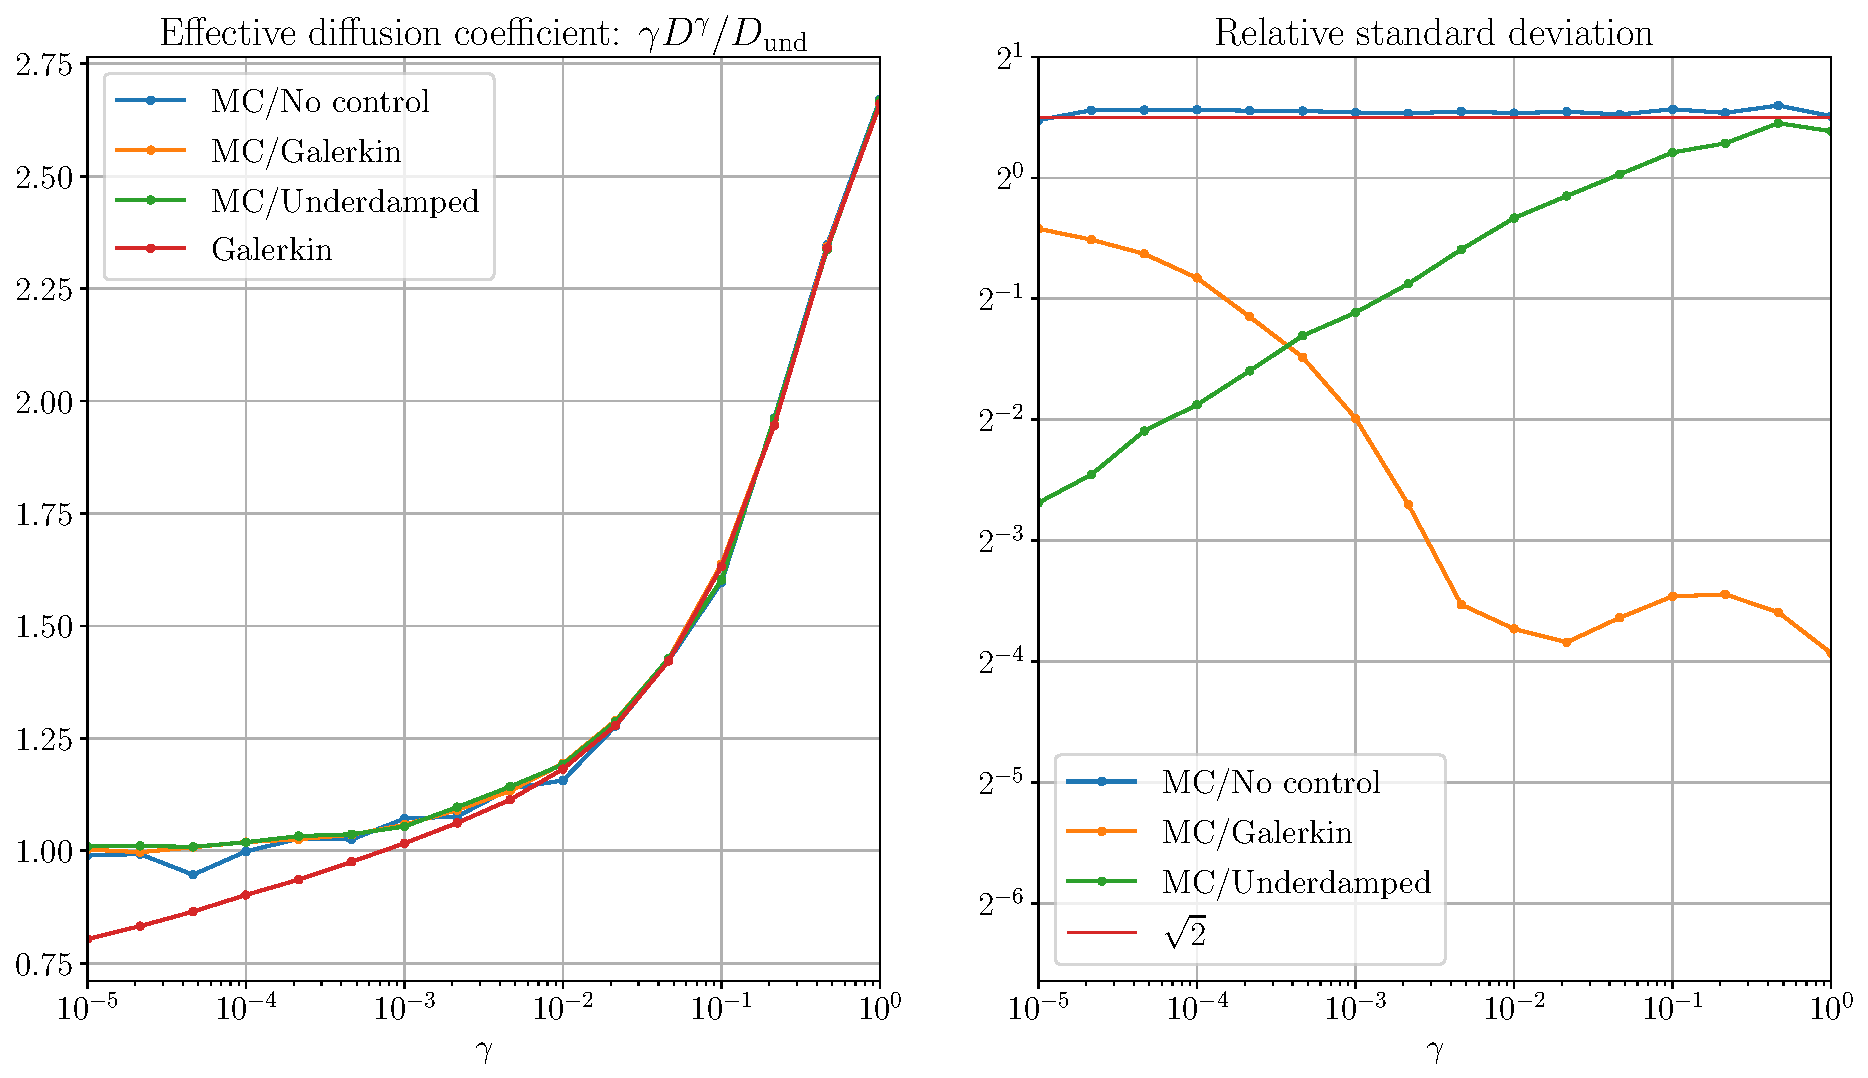
\includegraphics[width=0.99\linewidth]{figures/underdamped_1d.pdf}
    \caption{
        Effective diffusion coefficient and standard deviation of the estimators considered.
        The data labeled ``MC/No control'' correspond to Monte Carlo simulations without a control variate,
        i.e.\ to the estimator $u(T)$ given in~\eqref{eq:simple_estimator}.
        The data labeled ``MC/Galerkin'' and ``MC/Underdamped'' correspond to the improved estimator~\eqref{eq:definition_control_variate},
        with $\psi$ obtained using the approaches of~\cref{sub:galerkin_approach} and~\cref{sub:underdamped_approach},
        respectively.
        Finally, the curve labeled ``Galerkin'' is the approximate diffusion coefficient obtained by the Galerkin method,
        which is given by $\ip*{\widehat \Phi_N}{p}$ in the notation of \cref{sub:galerkin_approach}.
    }%
    \label{fig:effective_diffusion_langevin}
\end{figure}

\Cref{fig:time_bias_variance} illustrates the evolution of the expectation and standard deviation of the estimators~$u(t)$ and~$v(t)$,
estimated from 5000 trajectories,
with respect to the integration time $t$.
It appears clearly that,
for the value $\gamma = 10^{-3}$ considered,
the improved estimators $v(t)$ corresponding to the approaches outlined in \cref{sub:galerkin_approach} and \cref{sub:underdamped_approach}
have a much smaller variance than $u(t)$ throughout the simulation.
\begin{figure}[ht]
    \centering
    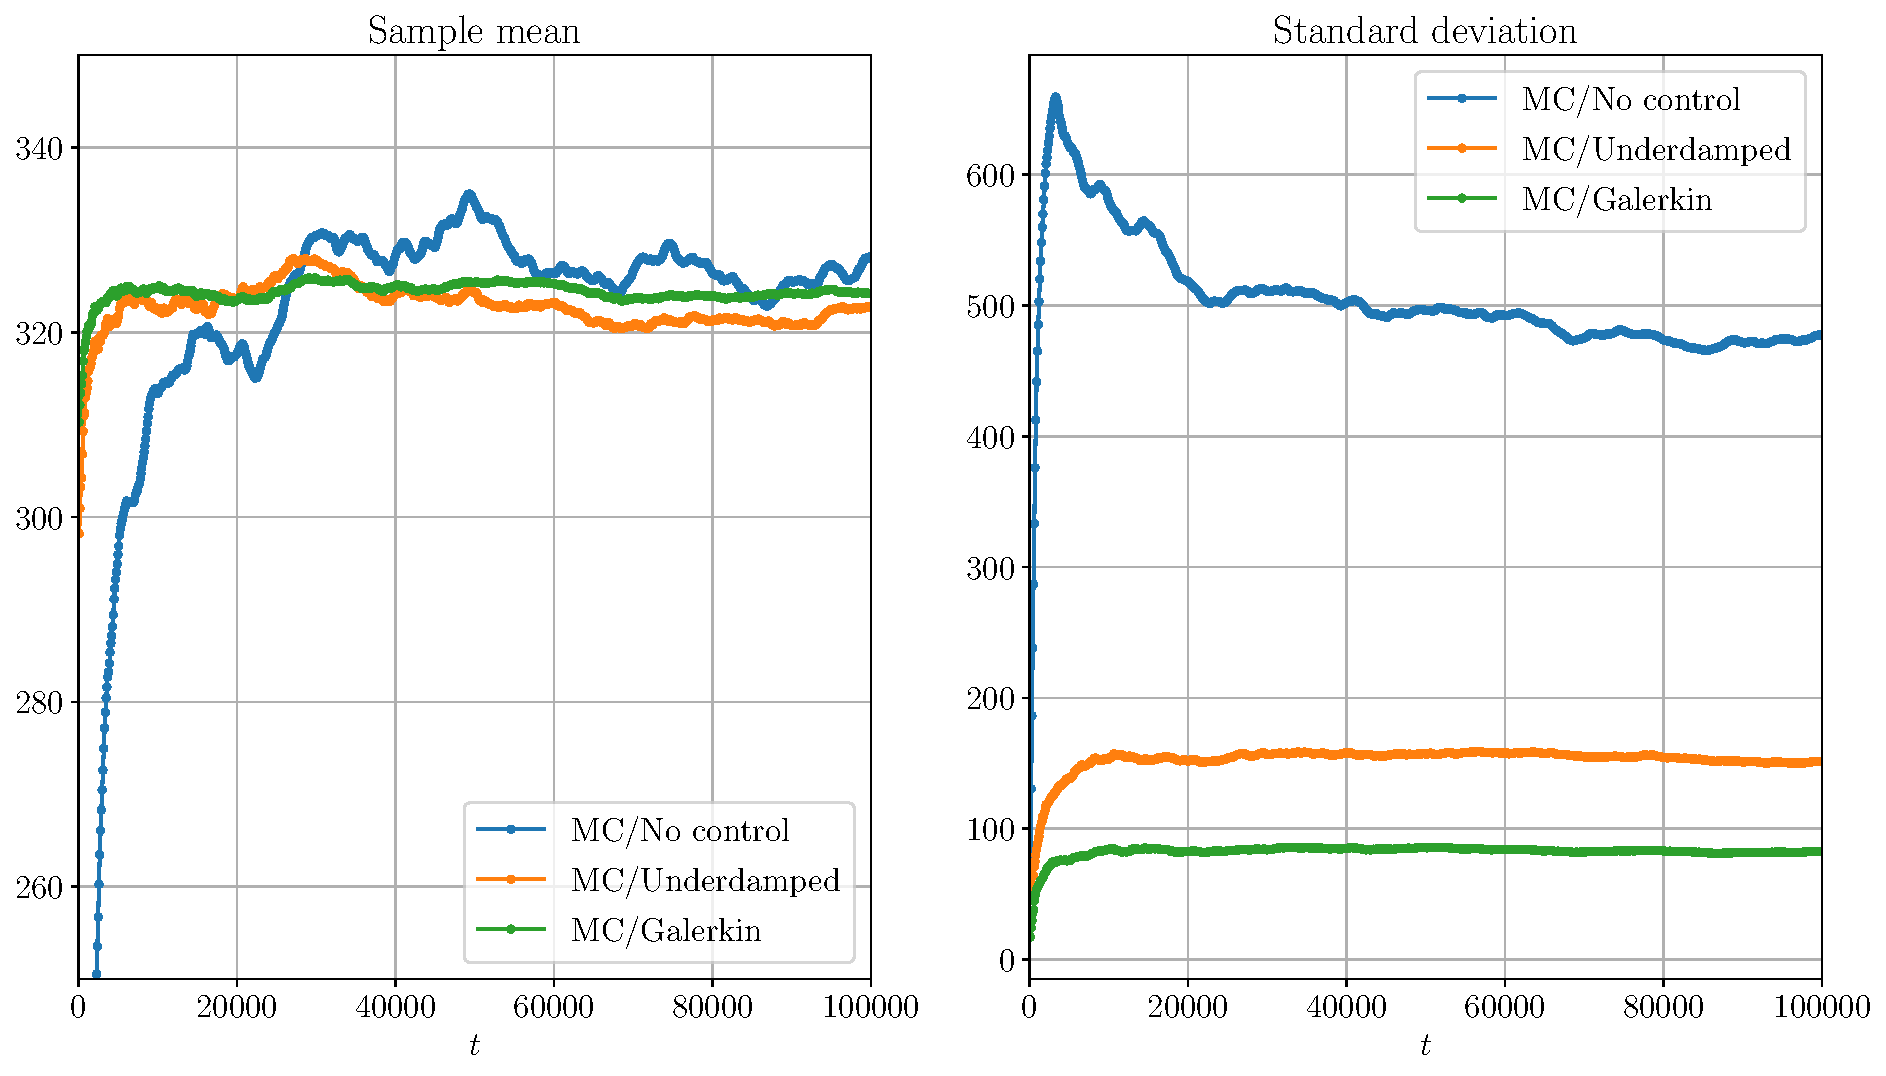
\includegraphics[width=0.99\linewidth]{figures/time.pdf}
    \caption{
        Sample mean and sample standard deviation of the estimators $u(t)$ and $v(t)$,
        for the friction parameter $\gamma = 10^{-4}$.
        The approximate solution to the Poisson equation used for constructing the control variate appearing in $v(t)$ here
        is that given in \cref{sub:underdamped_approach}.
    }%
    \label{fig:time_bias_variance}
\end{figure}

\subsection{Extension to generalized Langevin dynamics}%
\label{sub:generalization_to_generalized_langevin_dynamics}
The variance reduction approach described in \cref{sec:method},
in particular with the control variate constructed from the limiting solution to the Poisson equation as $\gamma \to 0$,
may be extended for calculating the mobility of simple generalized Langevin dynamics in one spatial dimension.
The paradigmatic example dynamics we consider here is the following,
which is studied in~\cite{MR2793823,GPGSUV21}:
\begin{equation}
\label{eq:gle}
\left\{
  \begin{aligned}
      & \d q_t = p_t \, \d t, \\
      & \d p_t = - V'(q_t) \, \d t + \frac{\sqrt{\gamma}}{\nu} \, z_t \, \d t, \\
      & \d z_t = - \frac{\sqrt{\gamma}}{\nu} \, p_t  \, \d t
       -   \frac{1}{\nu^2} \, z_t \, \d t + \sqrt{\frac{2\beta^{-1}}{\nu^2}} \, \d W_t.
  \end{aligned}
\right.
\end{equation}
A functional central limit theorem applies also to this dynamics:
the diffusively rescaled position process $(\varepsilon q_{t/\varepsilon^2})_{t \geq 0}$ converges in distribution,
in the Banach space of continuous functions over a bounded time interval,
to a Brownian motion with prefactor $\sqrt{2 D^{\gamma, \nu}}$.
Like Langevin dynamics, generalized Langevin dynamics are difficult to understand in the underdamped regime,
and in particular there does not exist a rigorous result on the behavior of $D^{\gamma, \nu}$ in the limit as $\gamma \to 0$.
Our goal in this section is to calculate accurately the mobility for the dynamics~\eqref{eq:gle} in the underdamped regime
using a control variate approach similar to that described in~\cref{sec:method},
and to assess in this way the validity of the asymptotic scaling of $D^{\gamma,\nu}$ conjectured in~\cite{GPGSUV21} by means of formal asymptotics.
An application of It\^o's formula gives
\[
    q_T - q_0 = \int_{0}^{T} p_t \, \d t
    = \phi(q_0, p_0) - \phi(q_t, p_t) + \sqrt{\frac{2 \beta^{-1}}{\nu^2}} \int_{0}^{T} \partial_z \phi(q_t, p_t) \, \d t,
\]
where $\phi$ is now the solution to the Poisson equation $- \mathcal L_{\rm GLE} \phi = p$,
with $\mathcal L_{\rm GLE}$ the generator of~\eqref{eq:gle}.
This suggests using the following estimator for the mobility:
\begin{subequations}
\begin{equation}
    \label{eq:improved_estimator_gle}
    v(T) = d_{\psi}+ \frac{1}{2T} \left( \abs*{q_T - q_0}^2 - \abs{\xi_T}^2\right),
\end{equation}
where $d_{\psi} := \sqrt{\frac{2 \beta^{-1}}{\nu^2}} \int \abs{\partial_z \psi}^2 \, \d \mu_{\rm GLE}$ and
\begin{align}
    \label{eq:definition_control_variate_gle}
    \xi_T = \psi(q_0, p_0) - \psi(q_T, p_T) + \sqrt{\frac{2 \beta^{-1}}{\nu^2}} \int_{0}^{T} \partial_z \psi(q_t, p_t) \, \d W_t,
\end{align}
\end{subequations}
for an approximate solution $\psi$ to the Poisson equation.
Here $\mu_{\rm GLE}(\d x) \propto \exp \left( - H(q,p) + \frac{z^2}{2}\right) \, \d x$ is the invariant probability distribution of~\eqref{eq:gle}.

In~\cite{GPGSUV21},
we employ an asymptotic expansion of the form
\(
    \phi = \gamma^{-1} \phi_0 + \gamma^{-1/2} \phi_1 + \gamma^{-1} \phi_2 \cdots
\)
in order to study the underdamped limit,
and we derive expressions for $\phi_0$ and $\phi_1$
which enable to formally show that $D^{\gamma, \nu}$ behaves as $\gamma^{-1}$ in the limit as $\gamma \to 0$,
with a prefactor that can be calculated efficiently and is different from $D_{\rm und}$.
Although the assumed asymptotic is shown to be invalid in~\cite{MR1088478},
our numerical results in this section demonstrate that this expansion can be leveraged for constructing an efficient control variate in~\eqref{eq:definition_control_variate_gle}.
Specifically,
we obtain a considerable variance reduction by letting $\psi = \gamma^{-1} \phi_0 + \gamma^{-1/2} \phi_1$.
We refer to~\cite{GPGSUV21} for the expressions of the $\phi_0$ and $\phi_1$.

\Cref{fig:effective_diffusion_time_gle} illustrates the evolution of $\expect u(t)$ and $\expect v(t)$ with respect to time,
for a value of $\nu = 2$ that is sufficiently large to observe differences with standard Langevin dynamics.
These expectations are estimated from 5000 trajectories,
and the associated $99.7\%$ confidence intervals (assuming Gaussianity) are depicted.
It is evident from the figures that the control variate enables considerable improvements,
both in terms of bias and variance.
Furthermore, we observe that the effective diffusion coefficient for $\gamma = 10^{-5}$
is in very good agreement with the limit conjectured in~\cite{GPGSUV21}.
The evolution of the effective diffusion with respect to $\gamma$ is presented in~\cref{fig:effective_diffusion_gle}.
\begin{figure}[ht]
    \centering
    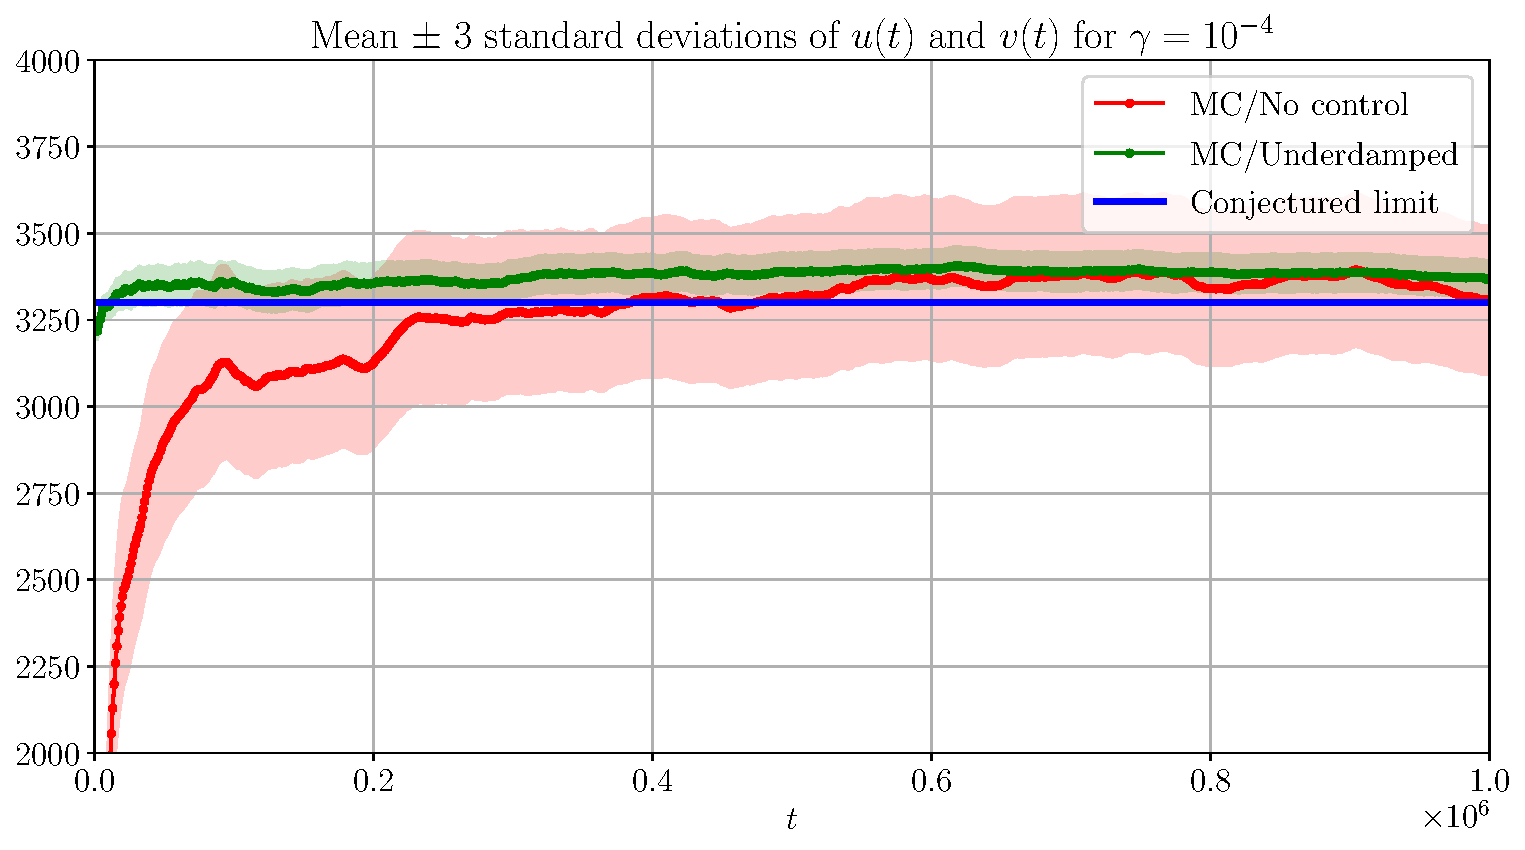
\includegraphics[width=0.495\linewidth]{figures/time-gle-4.pdf}
    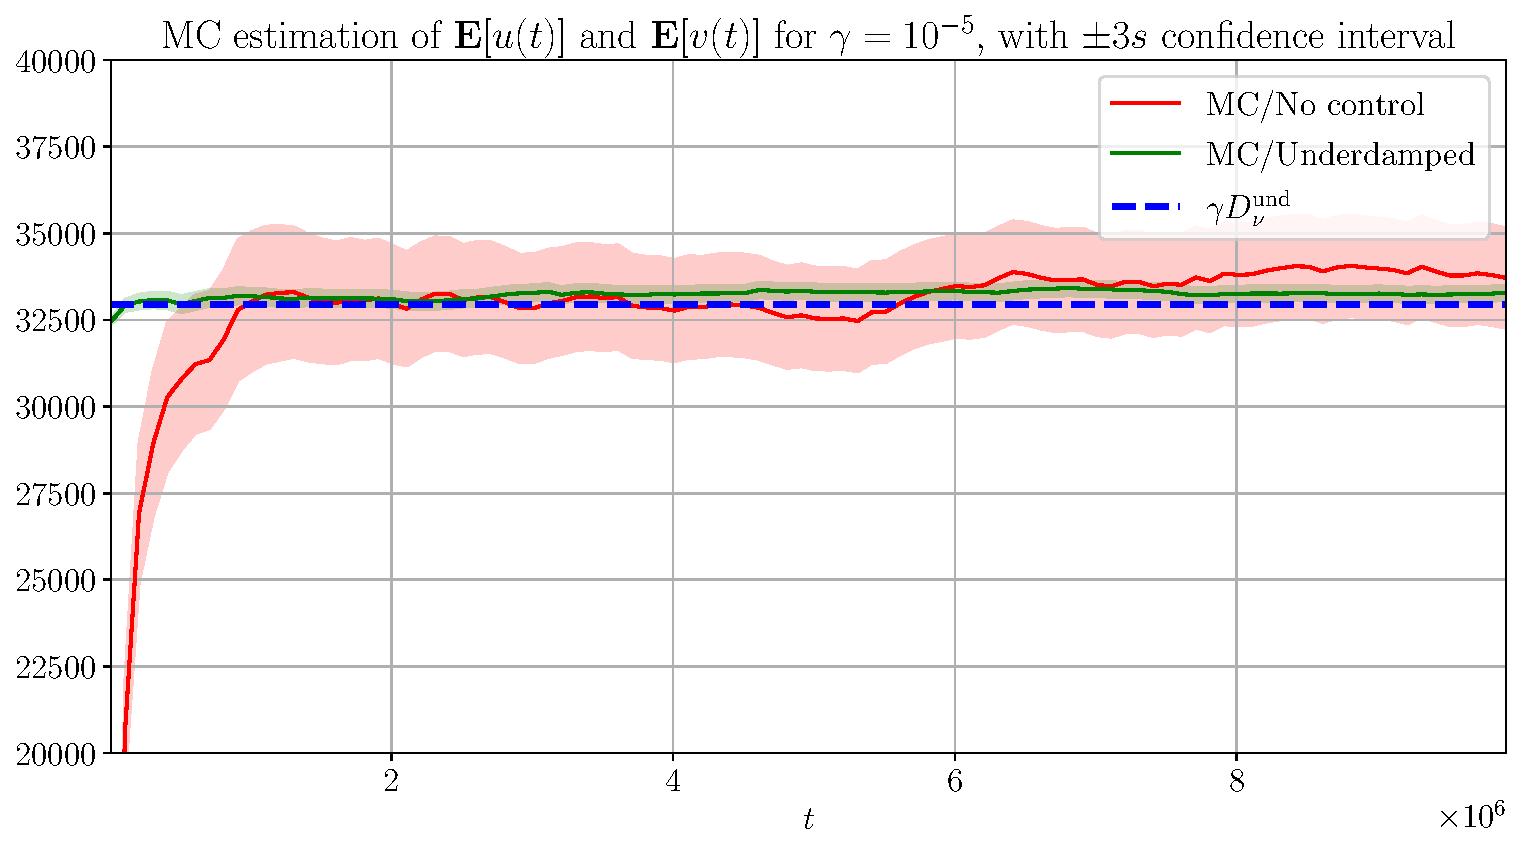
\includegraphics[width=0.495\linewidth]{figures/time-gle-5.pdf}
    \caption{%
        Expectations of the naive~\eqref{eq:simple_estimator} and improved~\eqref{eq:improved_estimator_gle} estimators for generalized Langevin dynamics
        and associated confidence $99.7\%$ intervals,
        estimated from $5000$ trajectories.
    }
    \label{fig:effective_diffusion_time_gle}
\end{figure}
\begin{figure}[ht]
    \centering
    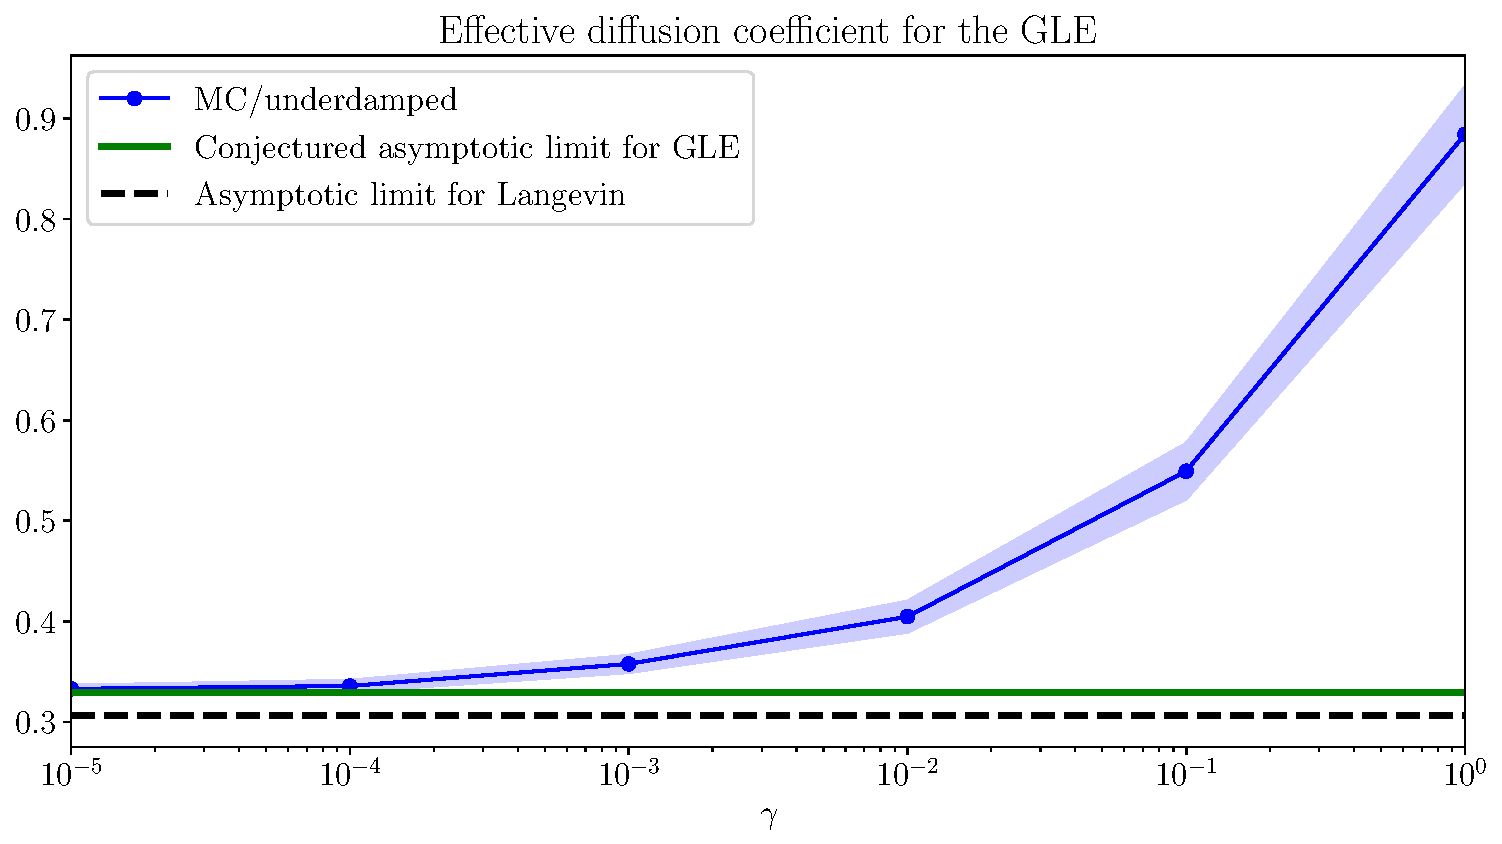
\includegraphics[width=0.75\linewidth]{figures/mobility_gle.pdf}
    \caption{%
        Expectation and $99.7\%$ confidence intervals for $v(T)$ in the underdamped limit,
        in the case of generalized Langevin dynamics with $\nu = 2$.
        Since $T$ scales as $1/\gamma$ with a large prefactor,
        it is expected that $\expect v(T) \approx D^{\gamma,\nu}$.
    }
    \label{fig:effective_diffusion_gle}
\end{figure}


% An alternative viewpoint on the control variate approach presented in \cref{sub:galerkin_approach} is that
% Monte Carlo simulation is employed in order to refine estimates obtained by Fourier/Hermite spectral method for the Poisson equation~\eqref{eq:poisson_equation}.

\section{Application to Langevin dynamics in two dimensions}%
\label{sec:applications_2d}%
The approaches employed in \cref{sec:application_to_one_dimensional_langevin_type_dynamics} for constructing an approximate solution to the Poisson equation~\eqref{eq:poisson_equation}
do not generalize well to the multi-dimensional setting for non-separable potentials.
On one hand, Galerkin methods for the Poisson equation suffer from the curse of dimensionality and,
on the other hand, the behavior of the solution to the Poisson equation is not well understood in the underdamped limit.
In this section we discuss alternative approaches.
We consider in this work a non-separable potential even simpler than~\eqref{eq:potential_julien}:
\begin{align*}
    \label{eq:potential_simple}
    V(q) =  v(q_1) + v(q_2) - \delta w(q_1, q_2) := - \cos(q_1) - \cos(q_2) - \delta \cos(q_1) \cos(q_2).
\end{align*}
In view of the symmetry of this potential,
the diffusion tensor is a multiple of the identity,
so we can focus on estimating $D^{\gamma}_{\vect e}$ only for the unit vector $\vect e = (1, 0)^\t$,
which simplifies the discussion.
Let $\phi_1(q, p)$ denote the solution to the Poisson equation $- \mathcal L \phi_1 = p_1$,
where the generator~$\mathcal L$ of the dynamics now reads
\[
    \mathcal L = L_1 + L_2
    + \delta \bigl( -\sin(q_1) \cos(q_2) \, \partial_{q_1} - \cos(q_1) \sin (q_2) \, \partial_{q_2} \bigr),
\]
with $L_i = p_i \partial_{q_i} - v'(q_i) \, \partial_{p_i} + \gamma \left(- p_i \partial_{p_i} + \beta^{-1} \partial^2_{p_i} \right)$,
for $i \in \{1, 2\}$.
Notice that $\phi_1(q, p) = \phi(q_1, p_1)$ when $\delta = 0$,
where $\phi$ is the solution to the one-dimensional Poisson equation $-L_1 \phi(q_1, p_1) = p_1$.
Therefore, it is natural to use $\phi(q_1, p_1)$, or an approximation thereof,
as the function $\psi$ in the definition of the control variate~\eqref{eq:definition_control_variate}.

\begin{figure}[ht]
    \centering
    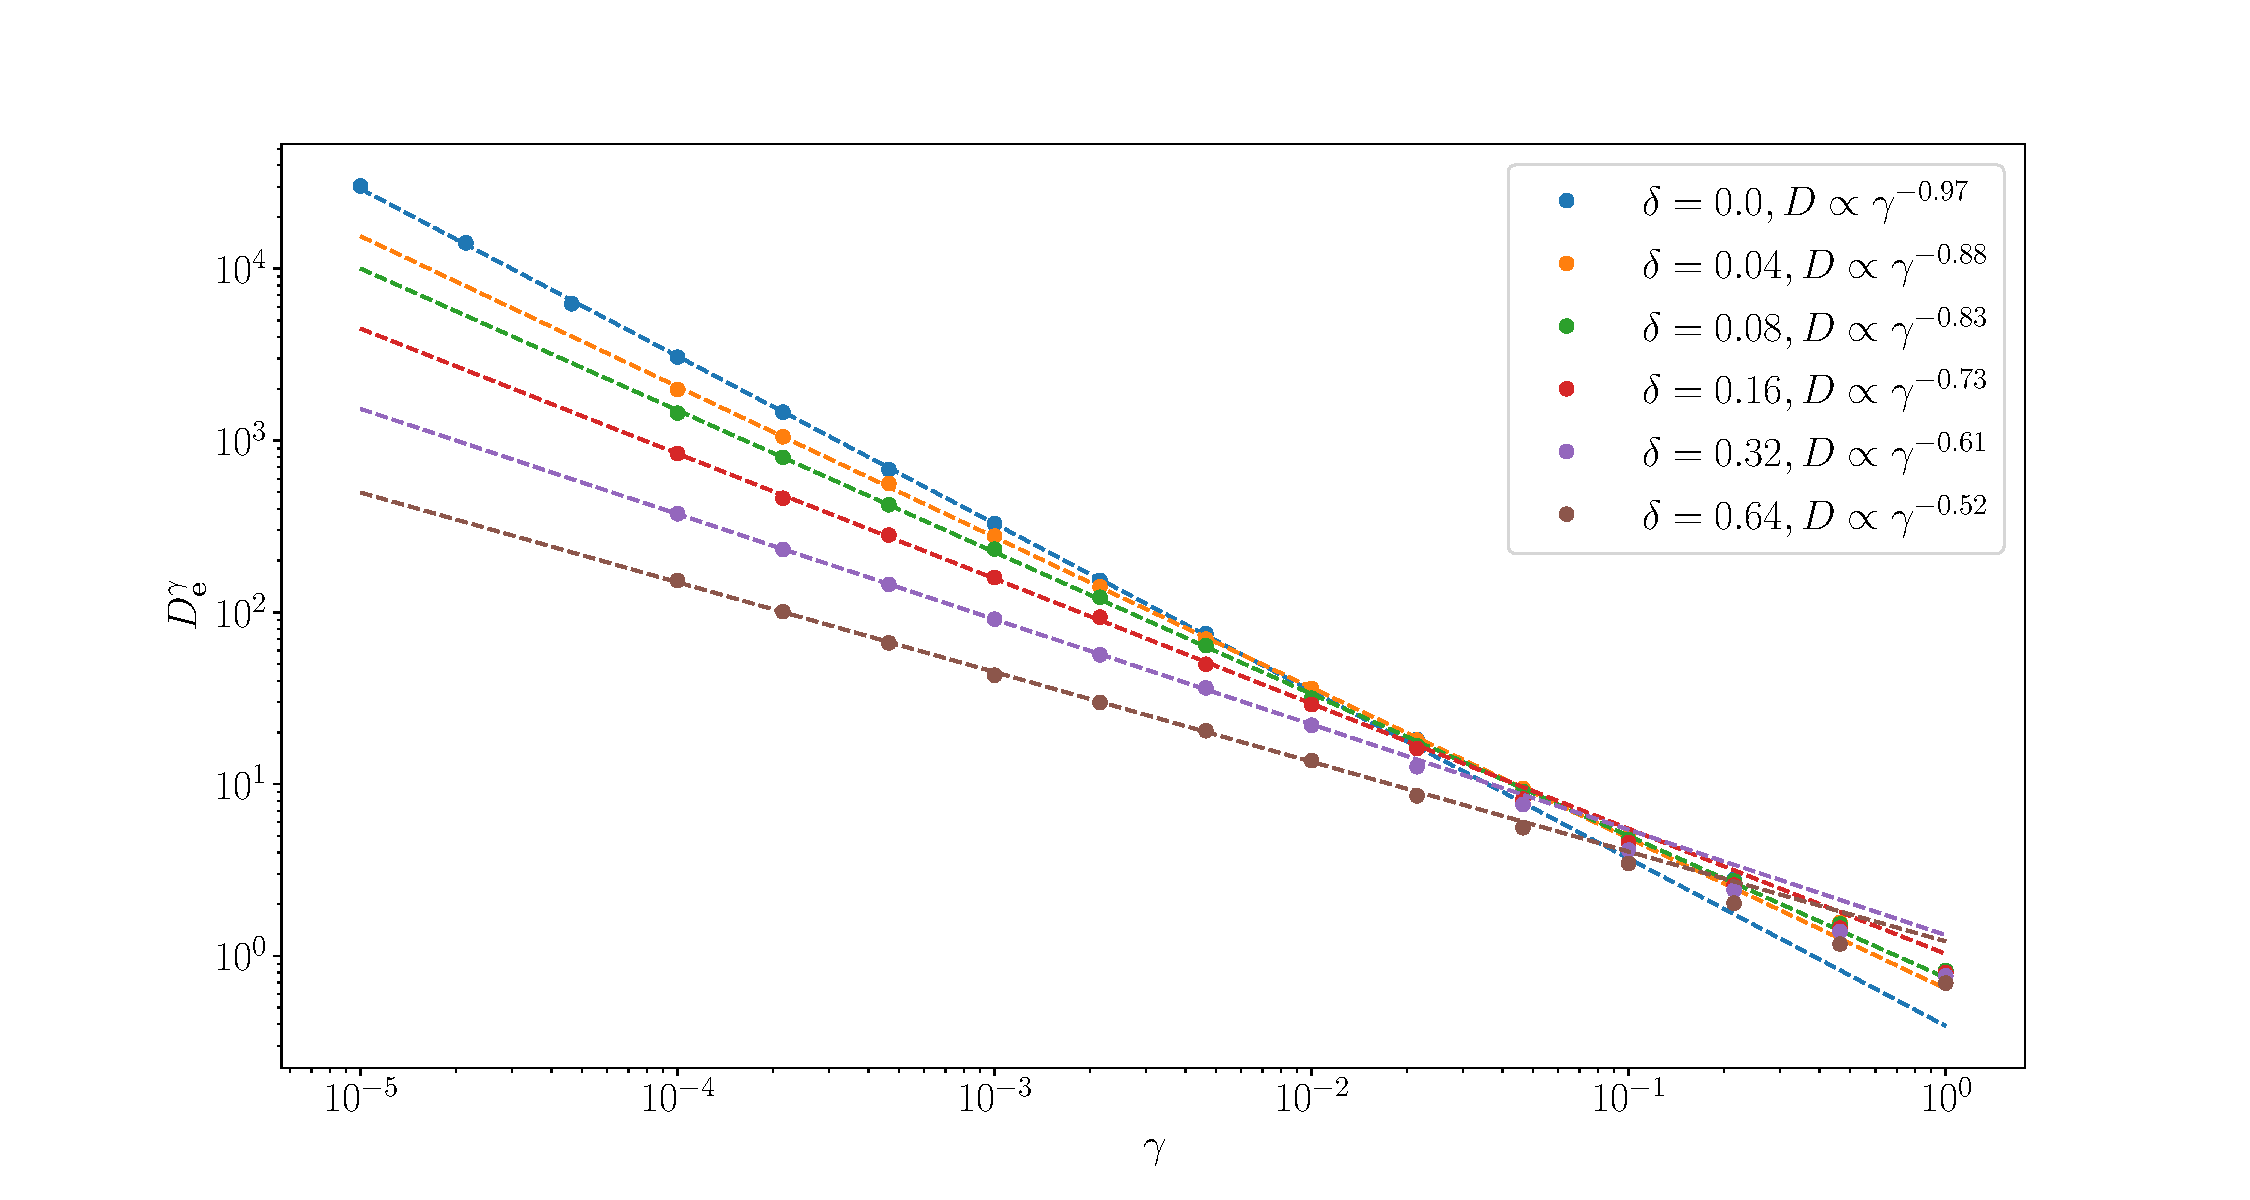
\includegraphics[width=0.99\linewidth]{figures/diffusion.pdf}
    \caption{
        Effective diffusion coefficient as a function of $\gamma$,
        for different values of $\delta$.
    }%
    \label{fig:time_bias_variance_2d}
\end{figure}
\begin{figure}[ht]
    \centering
    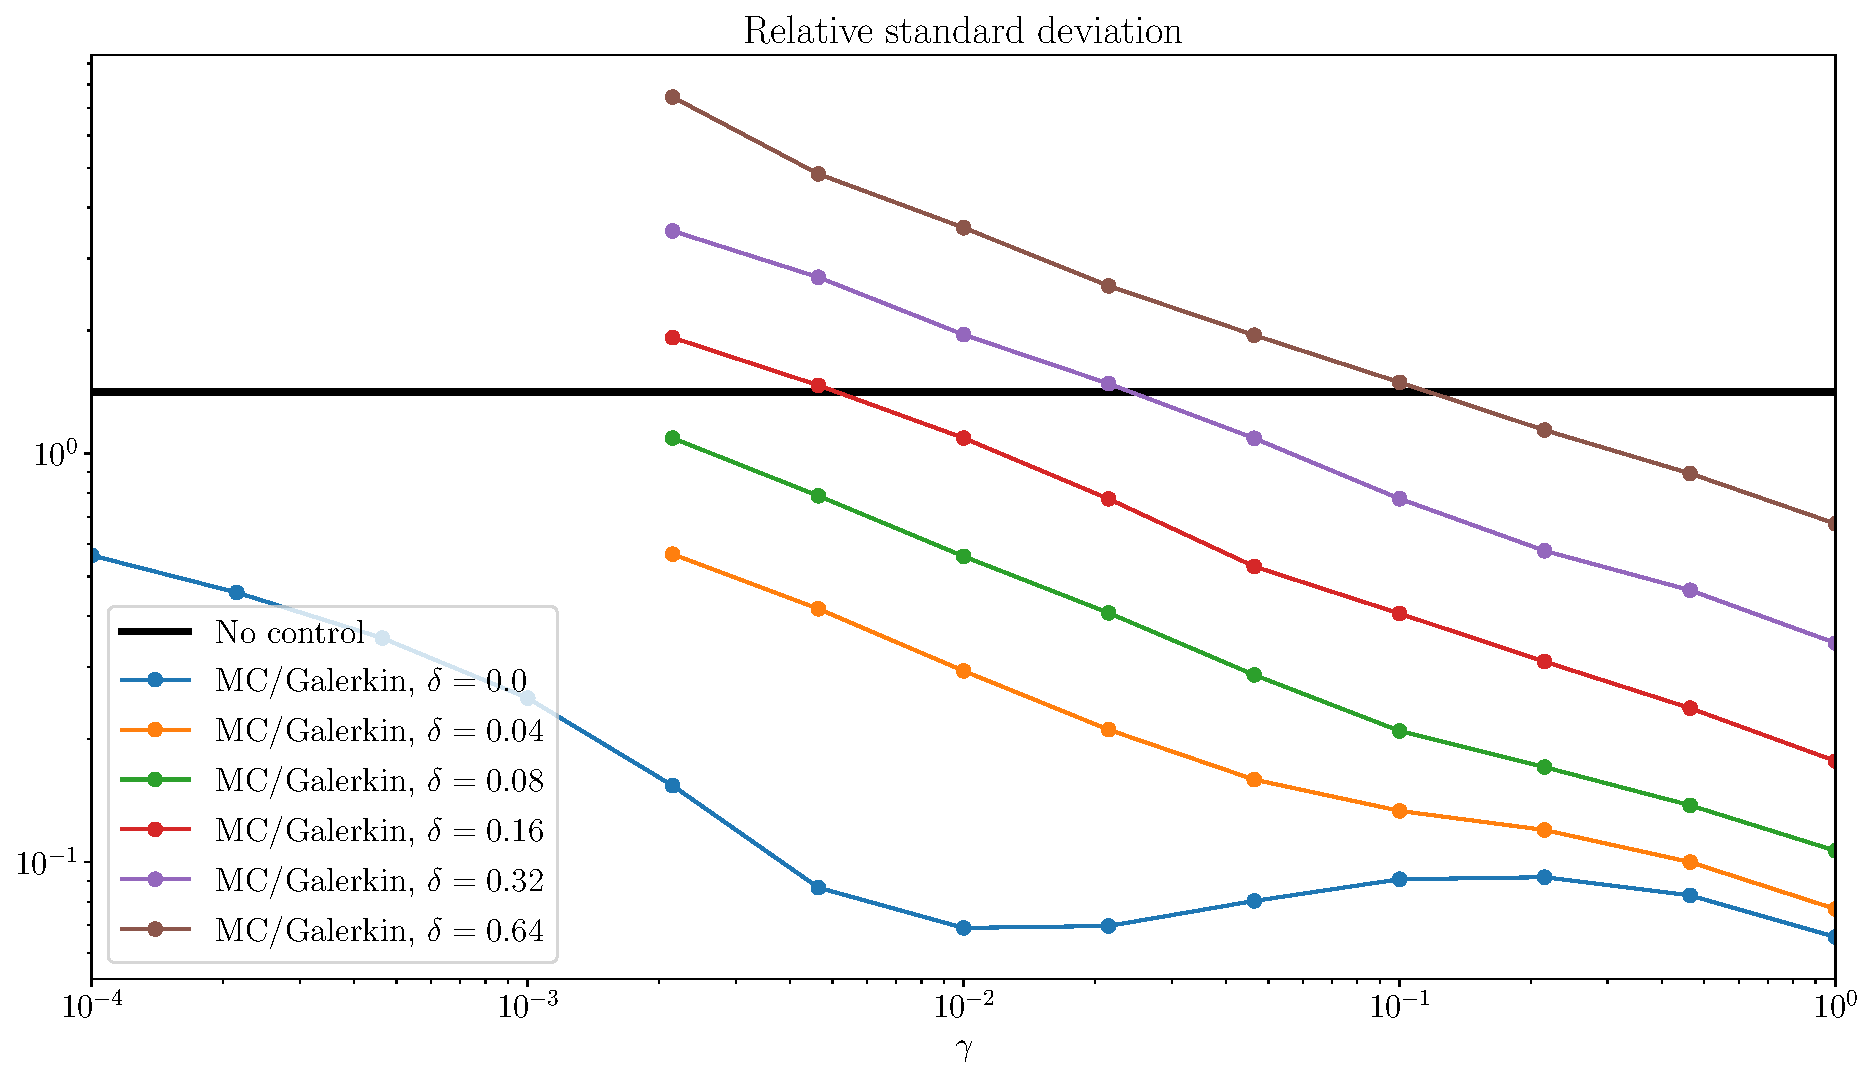
\includegraphics[width=0.49\linewidth]{figures/var-delta-galerkin.pdf}
    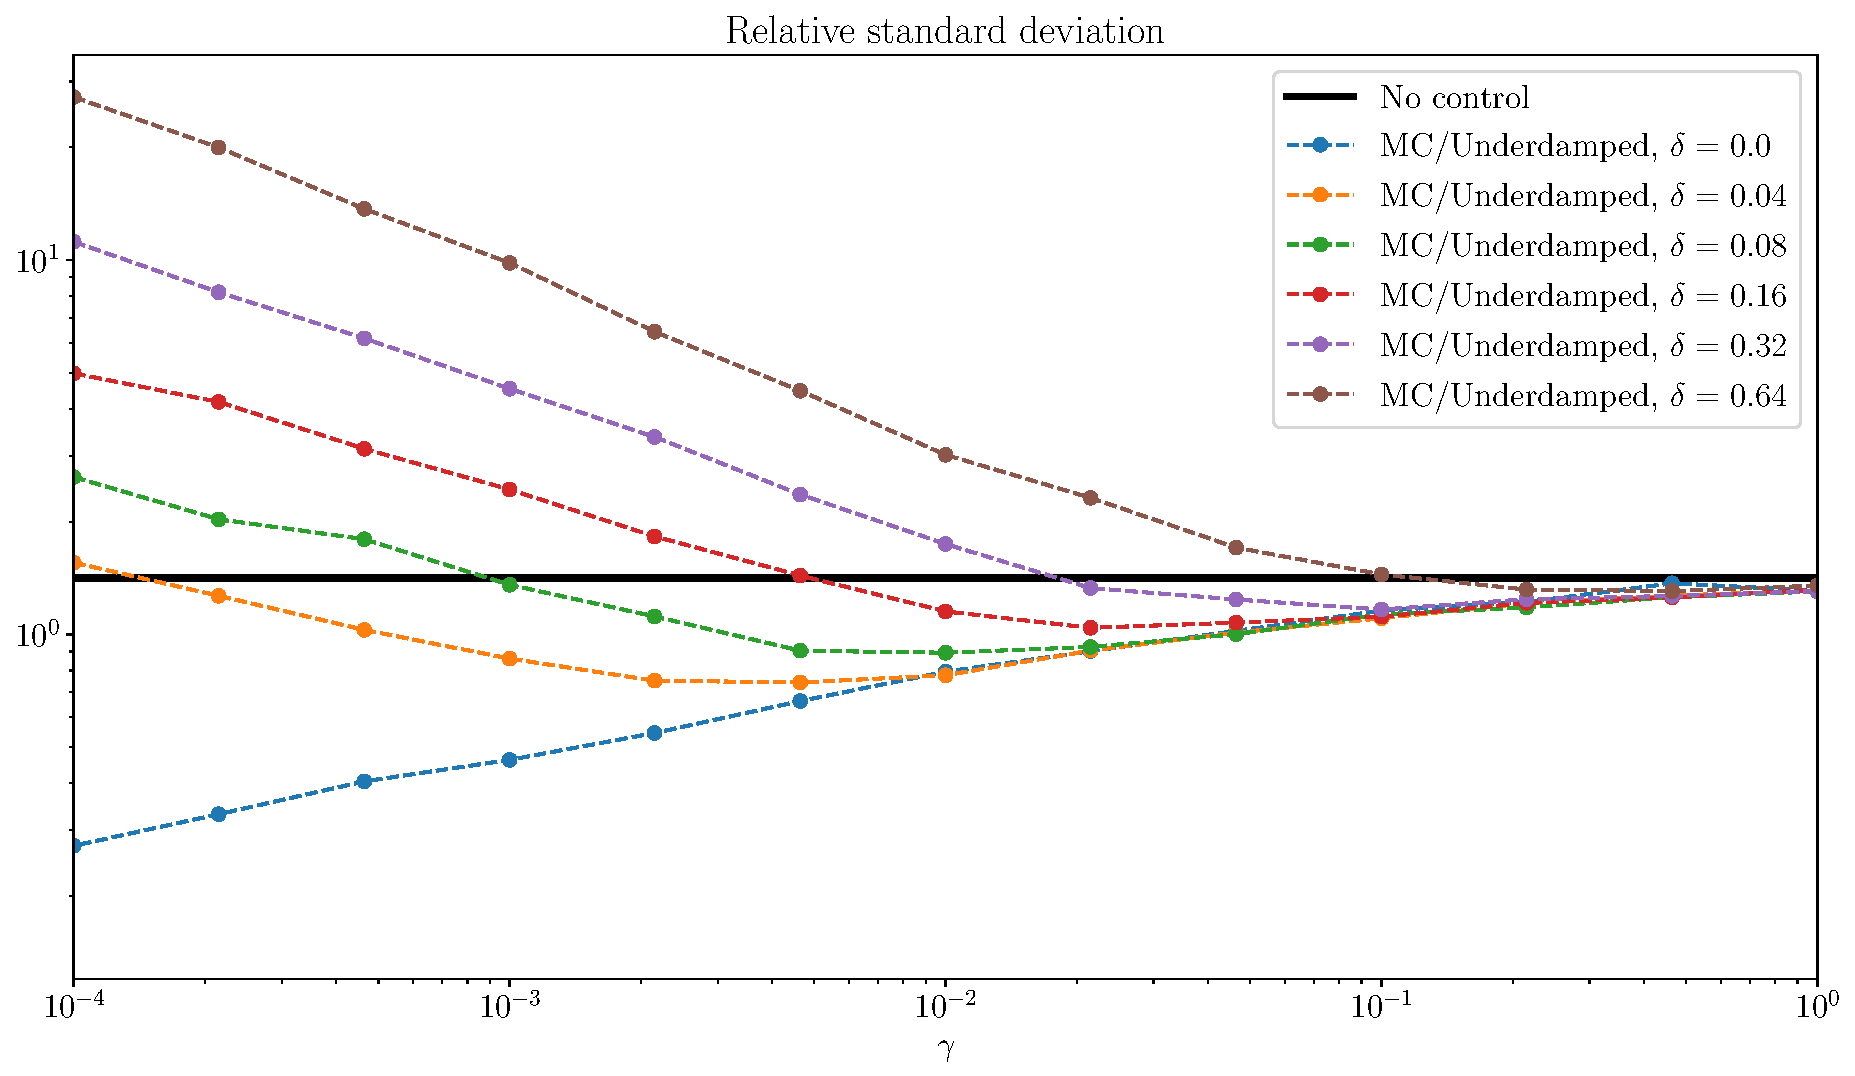
\includegraphics[width=0.49\linewidth]{figures/var-delta-underdamped.pdf}
    \caption{Relative standard deviation of the estimator $v(T)$.}%
\end{figure}

\section{Conclusions and perspectives for future work}%
\label{sec:conclusions_and_perspectives_for_future_work}
In this note,
we show how control variates techniques can be employed for improving estimators of the mobility of Langevin dynamics based on Einstein's formula.
The control variate approach we propose requires the knowledge of an approximate solution of a Poisson equation involving the generator of the dynamics.
We obtain general bounds on the bias and variance of the improved estimator in terms of the error on the solution to this equation,
and we study several practical approaches for constructing an approximate solution.

In the one-dimensional setting,
we demonstrate the efficiency of control variates
(i) obtained by a Fourier/Hermite spectral method and
(ii) based on an explicit expression for the limiting solution of the Poisson equation in the underdamped limit.
The latter approach, in particular,
leads to a variance reduction by a factor more than 10 for Monte Carlo methods in the very small friction regime $\gamma \leq 10^{-3}$,
in which purely deterministic Galerkin methods are typically inaccurate.

\appendix
\section{Proof of \texorpdfstring{\cref{proposition:semigroup_meanzero_observable}}{Proposition 2.1}}%
\label{sec:auxiliary_technical_results}

The proof is based on several lemmata.
In order to state the results, we first introduce some notation.
For a measure $\pi$, we define the weighted Sobolev space $H^i(\pi)$ as the subspace of $L^2(\pi)$
of functions whose derivatives up to order $i$ are in $L^2(\pi)$.
The associated norm is given by
\[
    \norm{u}_i^2 = \norm{f}^2 + \norm*{\nabla f}^2 + \dotsb + \norm*{\nabla^i f}^2,
\]
where  $\nabla^j f$ is the tensor containing the $j$-th order derivatives of $f$ and $\norm{\dummy}$ is the norm of~$L^2(\pi)$,
generalized to tensors in the usual manner.
We also define $H^{i}_0(\pi) = H^i(\pi) \cap L^2_0(\pi)$,
and we recall that a probability measure $\pi$ is said to satisfy the Poincaré inequality with constant $R$ if
\begin{equation}
    \label{eq:poincare}
    \tag{P$_R$}
    \forall f \in H^1_0(\pi), \qquad
    \norm*{f}^2 \leq \frac{1}{2R} \norm{\grad f}^2.
\end{equation}

% In the lemmata below, we focus on the periodic, one-dimensional case.
We also define $\nabla_q^* = \beta \nabla V(q) - \nabla_q$ and $\nabla_p^* = \beta p - \nabla_p$,
and note that these operators are formally the $L^2(\mu)$ adjoints of $\nabla_q$ and $\nabla_p$.
Similarly, in one dimension we write $\partial_q^* = \beta V'(q) - \partial_q$ and $\partial_p^* = \beta p - \partial_p$.
The first lemma is an application of standard elliptic theory and
concerns the exponential convergence of the derivatives of the overdamped Langevin semigroup.
\begin{lemma}
    \label{lemma:overdamped_langevin_decay_derivatives}
    Let $\mathcal X = \real^d$ or $\mathcal X = \torus^d$,
    and let $W: \mathcal X \to \real$ be a smooth potential such that the probability measure
    \[
        \pi(\d x) = \frac{\e^{- \beta W(x)} \d x}{\int_{\real^d} \e^{-\beta W(\widetilde x)} \d \widetilde x}
    \]
    satisfies~\eqref{eq:poincare}.
    Let also $\mathcal L_{\rm ovd}^W = - W'(p) \partial_p + \beta^{-1} \partial_p^2$ denote the generator of overdamped Langevin dynamics in potential~$W$.
    If $f \in H^i_0(\pi) \cap C^{\infty}(\mathcal X)$ for some $i \geq 0$,
    then $\e^{t \mathcal L_{\rm ovd}} f \in H^i_0(\pi)$ and there exists $K = K(i)$ such that
    \[
        \norm*{\e^{t \mathcal L_{\rm ovd}^W} f}_i \leq K \e^{- 2 R t} \norm*{f}_i.
    \]
\end{lemma}
\begin{proof}
    For simplicity, we consider only the case where $\mathcal X = \torus^d$,
    so that we know \emph{a priori} that~$\e^{t \mathcal L_{\rm ovd}^W} f \in H^i_0(\torus^d)$ because
    the state space is compact and $\e^{t \mathcal L_{\rm ovd}^W} f \in C^{\infty}(\torus^d)$ by ellipticity.
    To lighten notations,
    we also confine ourselves to the one-dimensional setting $d = 1$,
    but the proof carries over \emph{mutatis mutandis} to the multi-dimensional case.

    We use the notations $u(t) = \e^{t \mathcal L_{\rm ovd}^W} f$ and
     $\seminorm{h}_j = \norm*{(- \mathcal L_{\rm ovd}^W)^{j/2} h}$ for $j \geq 0$.
    Since $\mathcal L_{\rm ovd}^W$ commutes with~$(-\mathcal L_{\rm ovd}^W)^{i/2}$,
    it holds that
    \[
        \frac{1}{2} \derivative*{1}{t} \seminorm{u}_j^2 = \ip{\mathcal L_{\rm ovd}^W (-\mathcal L_{\rm ovd}^W)^{j/2} u}{(- \mathcal L_{\rm ovd}^W)^{j/2} u}.
    \]
    Introducing $\partial_x^* = \beta W' - \partial_x$
    and noting that $\mathcal L_{\rm ovd}^W = - \partial_x^* \partial_x$,
    we obtain
    \[
        \frac{1}{2} \derivative*{1}{t} \seminorm{u}_j^2 = - \norm*{\partial_x (-\mathcal L_{\rm ovd}^W)^{j/2} u}.
    \]
    Since $(-\mathcal L_{\rm ovd}^W)^{j/2} u \in L^2_0(\pi)$,
    we can apply Poincar\'e's inequality~\eqref{eq:poincare},
    which gives
    \[
        \frac{1}{2} \derivative*{1}{t} \seminorm{u}_j^2 \leq - 2R \seminorm{u}_j^2,
    \]
    implying the exponential convergence estimate
    \begin{equation}
        \label{eq:exponential_convergence}
        \forall t \geq 0, \qquad
        \seminorm{u(t)}_j \leq \e^{- 2 R t} \seminorm{u(0)}_j.
    \end{equation}
    Applying this estimate with $j = 0$ gives the usual convergence estimate for the norm $\norm{u}$.
    Since it holds for sufficiently regular $h$ that
    \[
        \seminorm{h}_1 = \norm*{(- \mathcal L_{\rm ovd}^W)^{1/2} h} = \sqrt{\ip{\mathcal L_{\rm ovd}^W h}{h}} = \beta^{-1} \norm{\partial_x h},
    \]
    equation~\eqref{eq:exponential_convergence} for $j = 1$ implies the exponential convergence of $\norm{\partial_x u}$.
    For $j = 2$, we calculate using the commutator relation $\commut{\partial_x}{\partial_x^*} = \beta V''$ that
    \[
        \seminorm{h}_2^2 = \norm*{- \mathcal L_{\rm ovd}^Wf}^2
        = \beta^{-2} \ip{\partial_x^* \partial_x h}{\partial_x^* \partial_x h}
        = \beta^{-2} \norm*{\partial_x^2 h}^2 + \beta^{-1} \ip{V'' \partial_x h}{\partial_x h}.
    \]
    Therefore~\eqref{eq:exponential_convergence} implies that
    \begin{align*}
        \norm*{\partial_x^2 u}^2
        &\leq \beta \abs{\ip{V'' \partial_x u}{\partial_x u}} + \e^{-4Rt} \bigl( \norm{\partial_x^2 u(0)}^2 + \beta \ip{V'' \partial_x u(0)}{\partial_x u(0)} \bigr) \\
        &\leq \beta \norm*{V''}_{\infty} \norm{\partial_x u}^2 + \e^{-4Rt} \bigl( \norm{\partial_x^2 u(0)}^2 + \beta \norm*{V''}_{\infty} \norm*{\partial_x u(0)}^2 \bigr),
    \end{align*}
    and using the exponential convergence of the first term on the right-hand side,
    which was proved in the previous step,
    allows to conclude that $\norm*{\partial_x^2 u} \leq K \e^{-2 Rt} \norm*{u}[2]$ for some appropriate constant $K \geq 1$.
    This procedure can then be repeated in order to deduce the statement.
\end{proof}

% \newcommand{\auxnorm}[1]{|\!|\!| #1 |\!|\!|}
% \begin{remark}
%     An alternative approach for showing~\cref{lemma:overdamped_langevin_decay_derivatives} is
%     to define an auxiliary norm
%     \[
%         \auxnorm{u}_N^2 = \norm*{u}^2 + a_1 \norm*{\partial_x u}^2 + \dotsc + a_N \norm*{\partial_x^N u}^2,
%     \]
%     with coefficients $a_i = \varepsilon^i$ for some $\varepsilon \in (0, 1)$.
%     This norm is equivalent to the weighted Sobolev norm $\norm*{u}_N$,
%     and it is possible to show for all $\lambda \in (0, 1)$ that
%     \[
%         \frac{1}{2}\derivative*{1}{t} \auxnorm{u}_N^2 \leq - 2 R(1 - \lambda) \, \auxnorm{u}_N^2
%     \]
%     for $\varepsilon$ sufficiently small.
%     The reason for the suboptimal rate here is that the term $\norm{\partial_x u}^2$,
%     obtained from $\frac{1}{2} \partial_t \norm*{u}^2$,
%     needs to control the two terms $\norm{u}^2 + a_1 \norm{\partial_x u}^2$.
% \end{remark}

For large times,
the derivatives of the semigroup can be controlled using only the $L^2(\mu)$ norm of the initial conditions.
We include the proof here for convenience.
\begin{lemma}
    [Elliptic regularization]
    \label{lemma:elliptic_reg}
    Let $(i,j) \in \nat^2$ with $j \leq i$.
    There exists a constant~$C_{ij}$ such that
    \[
        \forall t \in (0, 1], \qquad
        \norm*{\partial_x^i \e^{t \mathcal L_{\rm ovd}} f} \leq \frac{C_{ij}}{t^{\frac{i-j}{2}}} \norm*{f}[j]
    \]
\end{lemma}
\begin{proof}
    Let $u(t) = \e^{t \mathcal L_{\rm ovd}} f$.
    We will show the existence of constants $C_i$ such that
    \[
        \forall t \in (0, 1], \qquad
        \ip{(-\mathcal L)^i u(t)}{u(t)}
        \leq \frac{C_i}{t^{\frac{i-j}2}} \ip{(-\mathcal L)^j f}{f},
    \]
    after which the statement follows easily from the expression $\mathcal L = - \partial_x^* \partial_x$ and using commutations.
    Defining the Lyapunov functional
    \[
        N(t) = \sum_{n=j}^{i} \frac{t^{n-j}}{(n-j)!} \, \ip{(-\mathcal L)^n u(t)}{u(t)} ,
    \]
    we calculate
    \[
        N'(t) =  - \frac{t^{i-j}}{(i-j)!} \ip{(- \mathcal L)^{i+1} u(t)}{u(t)} \leq 0,
    \]
    which gives the statement since $N(0) = \norm{f}$.
\end{proof}

% The next lemma provides an estimate on the convergence of the solution to the backward Kolmogorov equation for Langevin dynamics
% in the overdamped limit $\gamma \to \infty$,
% in the case of an initial condition depending only on $q$.
% See also~\cite{MR496218,MR918689} for formal asymptotic expansions of the solution to the Fokker--Planck equation in the overdamped limit.
%
% \begin{lemma}
%     \label{lemma:backward_kolmogorov_obs_q}
%     Let $\mathcal L_{\rm ovd} = - V'(q) \partial_q + \beta^{-1} \partial_q^2$ and $f \in L^2_0(\nu) \cap C^{\infty}(\torus)$,
%     where $\nu$ is given in~\eqref{eq:definition_prob_measures}.
%     Let also $\bar f(q, p) = f(q)$ and
%     \[
%         \widehat u(t) = \e^{t\mathcal L_{\rm ovd}} f, \qquad
%         u(t) = \e^{t \gamma\mathcal L} \bar f.
%     \]
%     Then there exist positive constants $C$ and $\lambda$ independent of $f$ and $\gamma$ such that
%     \[
%         \forall \gamma \geq 1, \qquad
%         \forall t \geq 0, \qquad
%         \norm{u(t)  - \widehat u(t)} \leq
%         C \norm{f}_3 \gamma^{-1} \e^{-\lambda t}.
%     \]
% \end{lemma}
% \begin{proof}
%     Throughout this proof, $C$ denotes a positive constant that can change from occurrence to occurrence but is independent of $\gamma$ and $f$.
%     We recall that there exists a positive constant $\lambda_{\rm Lang}$ such that~\cite{roussel2018spectral,pavliotis2011applied}
%     \begin{equation}
%         \label{eq:decay_langevin}
%         \forall \gamma > 0, \qquad
%         \norm{\e^{t \gamma \mathcal L_{\rm Lang}}}[\mathcal B\left(L^2_0(\mu)\right)] \leq C \e^{- \lambda_{\rm Lang} \min\{1,\gamma^2\} t}.
%     \end{equation}
%     In addition, \cref{lemma:overdamped_langevin_decay_derivatives} implies the existence of $\lambda_{\rm ovd} > 0$ independent of $i$ such that
%     \begin{equation}
%         \label{eq:decay_ovd}
%         \norm{\e^{t \mathcal L_{\rm ovd}}}[\mathcal B\left(H^i_0(\mu)\right)] \leq C \e^{- \lambda_{\rm ovd} t}.
%     \end{equation}
%     Based on formal asymptotics expansions similar to those in~\cite[Chapter 6]{pavliotis2011applied},
%     we define the function
%     \(
%         \widetilde u(q, p, t) =
%         \widehat u(q, t)
%         + \gamma^{-1} p \, \partial_q \widehat u(q, t)
%         + \gamma^{-2} (p^2 - \beta^{-1}) \partial_q^{2} \widehat u.
%     \)
%     An explicit calculation gives
%     \begin{align*}
%         (\partial_t - \gamma \mathcal L) \widetilde u
%         &= \gamma^{-1} p \, \partial_t \partial_q \widehat u(q, t) + \gamma^{-2} (p^2 - \beta^{-1}) \partial_t \partial_q^{2} \widehat u
%         - \gamma^{-1} p (p^2 - \beta^{-1}) \partial_q^{3} \widehat u + 2 \gamma^{-1} p \, V'(q) \, \partial_q^2 \widehat u \\
%         &= - \gamma^{-1} p \, \partial_q \partial_q^* \partial_q \widehat u(q, t) - \gamma^{-2} (p^2 - \beta^{-1})  \partial_q^{2} \partial_q^* \partial_q \widehat u \\
%         &\qquad - \gamma^{-1} p (p^2 - \beta^{-1}) \partial_q^{3} \widehat u + 2 \gamma^{-1} p \, V'(q) \, \partial_q^2 \widehat u.
%     \end{align*}
%     The right-hand side, which we denote by $\gamma^{-1} r(t)$, has values in $L^2_0(\mu)$.
%     By the general Leibniz rule gives,
%     it is simple to show that
%     \begin{equation}
%         \label{eq:commutators_derivatives}
%         \commut{\partial_q^N}{\partial_q^*}
%         = \commut{\partial_q^N}{\beta V' - \partial_q}
%         = \beta \commut{\partial_q^N}{V'}
%         = \beta \sum_{k=1}^{N} {N \choose k} V^{(k+1)} \partial_q^{(N-k)},
%     \end{equation}
%     which can be employed to show that $\norm{r(t)} \leq C \norm{\widehat u(t)}_4$.
%     Using~\cref{lemma:overdamped_langevin_decay_derivatives,lemma:elliptic_reg},
%     we deduce that
%     \begin{align}
%         \label{eq:bound_remainder}
%         \norm{r(t)} \leq \frac{C}{\sqrt{\min(t, 1)}}  \e^{- \lambda_{\rm ovd} \, \max(t-1, 0)} \norm{f}[3]
%     \end{align}
%     % and so $\norm{r(t)} \leq C \e^{-\lambda_{\rm ovd} t} \norm{f}_4$ by~\eqref{eq:decay_ovd}.
%     Using the notation $e(t) = u(t) - \widetilde u(t)$,
%     we calculate that $e$ satisfies the equation
%     \[
%         \partial_t e = \gamma \mathcal L e - \gamma^{-1} r, \qquad
%         e(0) = \gamma^{-1} p \, f'(q) + \gamma^{-2} (\beta^{-1} - p^2) f''(q).
%     \]
%     By Duhamel's formula,
%     this implies
%     \[
%         e(t) = \e^{t \gamma \mathcal L} \bigl( e(0) \bigr) + \gamma^{-1} \int_{0}^{t} \e^{(t- s) \gamma \mathcal L} r(s) \, \d s.
%     \]
%     From~\eqref{eq:decay_langevin} and~\eqref{eq:bound_remainder} we deduce immediately that
%     \begin{align*}
%         e(t)
%         &\leq C \e^{- \lambda_{\rm Lang} t} \norm{e(0)}
%         + C \gamma^{-1} \norm{f}[3] \int_{0}^{t} \e^{- \lambda_{\rm Lang} (t-s)} \frac{1}{\sqrt{\min(s, 1)}}  \e^{- \lambda_{\rm ovd} \, \max(s-1, 0)} \d s \\
%         &\leq C \e^{- \lambda t} \norm{e(0)} + C \norm{f}_3 \gamma^{-1} \e^{- \lambda t},
%     \end{align*}
%     for $\lambda = \min(\lambda_{\rm ovd}, \lambda_{\rm Lang})$.
%     The result then follows after noticing that $\norm{e(0)} \leq C \gamma^{-1} \norm{f}_2$ and
%     \[
%         \norm{\widetilde u(t) - \widehat u(t)} \leq C \norm{f}_2 \gamma^{-1} \e^{- \lambda_{\rm ovd} t},
%     \]
%     by \eqref{eq:decay_ovd}.
% \end{proof}

The next lemma provides an intermediate result for proving~\cref{proposition:semigroup_meanzero_observable}.
The result proved here is sharper than what would be obtained from a simple application of~\eqref{eq:decay_semigroup_general},
but not yet sufficient for obtaining optimal estimates for the bias of estimator~\eqref{eq:simple_estimator}.
\begin{lemma}
    \label{lemma:initial_lemma}
    Assume that $f \in H^2(\mu)$ is a smooth function such that
    \begin{equation}
        \label{eq:assumption_f}
        \int f(q, p) \, \kappa(\d p) = 0.
    \end{equation}
    Then there exist constants $C$ and $\lambda$ independent of $\gamma$ and $f$ such that
    \[
        \forall \gamma > 1, \qquad
        \forall t \geq 0, \qquad
        \norm*{\e^{t\mathcal L} f}
        \leq C \bigl( \norm{f} + \norm{\partial_q f} \bigr)
        \left( \e^{- \gamma t} + \gamma^{-1} \e^{-\frac{\lambda t}{\gamma}} \right).
    \]
\end{lemma}
\begin{proof}
    We prove the result for functions $f(q, p)$ of the form
    \begin{equation}
        \label{eq:expansion}
        f(q, p) = \sum_{i=0}^{N} \sum_{j=1}^{N} c_{ij} \, G_i(q) H_j(p).
    \end{equation}
    where $G_i = {\rm Re}(\e^{ix})$ and $H_j$ denotes the Hermite polynomial of degree $j$.
    The space of functions of this form is dense in $(\id - \Pi_p) H^1(\mu)$,
    so the general result follows by density.

    % We consider the following decomposition of the generator:
    % \[
    %     \mathcal L
    %     = \left( p \derivative{1}{q} - \derivative*{1}[V]{q}(q) \derivative{1}{p} \right)
    %     + \gamma \left( - p \derivative{1}{p} + \beta^{-1} \derivative{2}{p^2} \right)
    %     =: \mathcal L_{\rm Ham} + \gamma \mathcal L_{\rm FD}.
    % \]
    Let $v(t) = \e^{t \mathcal L} f(q, p) - \e^{- t \gamma \mathcal L_{\rm FD}} f(q, p)$,
    where the operator $\mathcal L_{\rm FD}$ is defined in~\eqref{eq:decomposition_generator}.
    In the expression $\e^{- t \gamma \mathcal L_{\rm FD}} f(q, p)$,
    the variable $q$ should should be viewed as a parameter.
    The function~$v$ satisfies the initial value problem
    \[
        \partial_t v = \mathcal L v +  \mathcal L_{\rm Ham} \bigl(\e^{t \gamma \mathcal L_{\rm FD}} f\bigr), \qquad v(0) = 0.
    \]
    Using Duhamel's formula, we have
    \[
        v(t) = \int_{0}^{t} \e^{- (t-s) \mathcal L}  \Bigl( \mathcal L_{\rm Ham} \bigl(\e^{s \gamma \mathcal L_{\rm FD}} f\bigr) \Bigr) \, \d s,
    \]
    and therefore
    \begin{equation}
        \label{eq:intermediate_decay_correlation}
        \e^{t \mathcal L} f =  \e^{t \gamma \mathcal L_{\rm FD}} f
        + \int_{0}^{t} \e^{- (t-s) \mathcal L}  \Bigl( \mathcal L_{\rm Ham} \bigl(\e^{s \gamma \mathcal L_{\rm FD}} f\bigr) \Bigr) \, \d s.
    \end{equation}
    By~\eqref{eq:assumption_f} and with the notation $\norm{\dummy}[\kappa]$ for the norm of $L^2(\kappa)$,
    the first term is bounded as
    \begin{align}
        \notag
        \norm{\e^{t \gamma \mathcal L_{\rm FD}} f(q, p)}^2
        &= \int \!\!\!\! \int  \abs{\e^{t \gamma \mathcal L_{\rm FD}} f(q, p) }^2 \d \kappa(p) \,\d \nu(q)
        = \int \norm{\e^{t \gamma \mathcal L_{\rm FD}} f(q, \cdot) }[\kappa]^2 \, \d \nu(q) \\
        \label{eq:bound_first_term}
        &\leq \int \e^{-2 \gamma t} \norm{f(q, \cdot) }[\kappa]^2 \, \d \nu(q) = \e^{-2\gamma t} \norm{f}^2.
    \end{align}
    For the second term, since $\commut{\partial_p}{\partial_p^*} = \beta$ and $\commut{\partial_q}{\partial_q^*} = \beta V''$,
    we have
    \begin{align*}
        \norm{\partial_q \partial_p^* \e^{t \gamma \mathcal L_{\rm FD}} f}
        &= \norm{\partial_q \partial_p \e^{t \gamma \mathcal L_{\rm FD}} f} + \beta \norm{\partial_q \e^{t \gamma \mathcal L_{\rm FD}} f}, \\
        \norm{\partial_q^* \partial_p \e^{t \gamma \mathcal L_{\rm FD}} f}
        &= \norm{\partial_q \partial_p \e^{t \gamma \mathcal L_{\rm FD}} f}
        + \beta \ip{V''(q) \partial_p \e^{t \gamma \mathcal L_{\rm FD}} f}{\partial_p \e^{t \gamma \mathcal L_{\rm FD}} f} \\
        &\leq \norm{\partial_q \partial_p \e^{t \gamma \mathcal L_{\rm FD}} f}
        + \beta \norm{V''}[\infty] \norm{\partial_p \e^{t \gamma \mathcal L_{\rm FD}} f}.
    \end{align*}
    From these equations we deduce
    \begin{align}
        \notag
        \norm{\mathcal L_{\rm Ham} \e^{t \gamma \mathcal L_{\rm FD}} f}
        &= \beta^{-1} (\partial_q \partial_p^* - \partial_q^* \partial_p) \e^{t \gamma \mathcal L_{\rm FD}} f \\
        \label{eq:reasoning_action_lham}
        &\leq 2 \beta^{-1} \norm{\partial_q \partial_p \e^{t \gamma \mathcal L_{\rm FD}} f}
        + \norm{\partial_q \e^{t \gamma \mathcal L_{\rm FD}} f}
        + \norm*{V''}[\infty] \norm{\partial_p \e^{t \gamma \mathcal L_{\rm FD}} f}.
    \end{align}
    Since $f$ is assumed to be a finite linear combination of the form~\eqref{eq:expansion} and
    Hermite polynomials are the eigenfunctions of $\mathcal L_{\rm FD}$,
    we can freely change the order of the operators $\partial_q$ and $\e^{t \gamma \mathcal F_{\rm FD}}$.
    % Since $\mathcal L_{\rm FD}$ is not hypoelliptic when viewed as an operator acting on functions of $q$ and $p$,
    % it is not clear \emph{a priori} that~$\e^{t \gamma \mathcal L_{\rm FD}} f$ is a smooth function.
    From \cref{lemma:overdamped_langevin_decay_derivatives}, the fact that $\kappa$ satisfies~\eqref{eq:poincare} with constant $R = \frac{1}{2}$,
    and \cref{lemma:elliptic_reg},
    we obtain
    \begin{align}
        \label{eq:bound_action_lham}
        \norm{\mathcal L_{\rm Ham} \e^{t \gamma \mathcal L_{\rm FD}} f}
        &\leq C \left( \frac{\e^{-\gamma t}}{\sqrt{1 \wedge \gamma t}} \right) \bigl( \norm{f} + \norm{\partial_q f} \bigr).
    \end{align}
    Going back to~\eqref{eq:intermediate_decay_correlation} and using~\eqref{eq:decay_semigroup_general},
    we obtain
    \begin{align*}
        \norm*{ \e^{t \mathcal L} f}
        &\leq  \e^{-\gamma t} \norm{f}
        + C  \bigl( \norm{f} + \norm{\partial_q f}\bigr) \int_{0}^{t} \e^{-\frac{\lambda_{\rm Lang}}{\gamma}(t-s)}  \, \left(\frac{\e^{-\gamma s}}{\sqrt{1 \wedge \gamma s}}\right) \, \d s.
    \end{align*}
    The integral can be bounded by decomposing the interval $[0, t]$ as $[0, \frac{1}{\gamma}] \cup [\frac{1}{\gamma}, t]$.
    \begin{align}
        \notag
        \int_{0}^{t} \e^{-\frac{\lambda_{\rm Lang}}{\gamma}(t-s)}  \, \left( \frac{\e^{-\gamma s}}{\sqrt{1 \wedge \gamma s}} \right) \, \d s
        & \leq
        \e^{-\frac{\lambda_{\rm Lang}}{\gamma} \left(t-\frac{1}{\gamma}\right)}
         \int_{0}^{\frac{1}{\gamma}}  \frac{1}{\sqrt{\gamma s\, }} \, \d s
         + \int_{\frac{1}{\gamma}}^{t} \e^{-\frac{\lambda_{\rm Lang}}{\gamma}(t-s) - \gamma s} \d s \\
         \notag
        & \leq
        \frac{2}{\gamma}\e^{-\frac{\lambda_{\rm Lang}}{\gamma} \left(t-\frac{1}{\gamma}\right)}
         + \int_{0}^{t} \e^{-\frac{\widetilde \lambda_{\rm Lang}}{\gamma}(t-s) - \gamma s} \d s
        \leq C  \gamma^{-1} \e^{-\frac{\widetilde \lambda_{\rm Lang} t}{\gamma}}.
    \end{align}
    where~$\widetilde \lambda_{\rm Lang} = \min \{\frac{1}{2}, \lambda_{\rm Lang} \}$.
    The conclusion then follows.
    % \begin{align*}
    %     &\leq  \e^{-\gamma t} \norm{f}
    %     + C \bigl( \norm{f} + \norm{\partial_q f} \bigr)
    %     \left( \frac{1}{\gamma} \e^{-\frac{\lambda_{\rm Lang}}{\gamma} t} + \frac{\e^{- \frac{\widetilde \lambda_{\rm Lang}}{\gamma}t} - \e^{- \gamma t}}{\gamma - \frac{\widetilde \lambda_{\rm Lang}}{\gamma}} \right) \qquad \forall \gamma \geq 1,
    % \end{align*}
    % which allows to conclude.
\end{proof}

We are now ready to prove~\cref{proposition:semigroup_meanzero_observable}.
\begin{proof}
    [Proof of \cref{proposition:semigroup_meanzero_observable}]
    We again show the result for functions of the form~\eqref{eq:expansion},
    noting that the general result follows by density of functions of this type in $\Pi_p^{\perp} L^2(\mu)$.
    From~\eqref{eq:intermediate_decay_correlation}, we obtain
    \begin{align}
        \notag
        \ip{\e^{t \mathcal L} f}{h}
        &= \ip{\e^{t \gamma \mathcal L_{\rm FD}} f}{h}
        + \int_{0}^t \ip{\e^{(t-s) \mathcal L} \Bigl( \mathcal L_{\rm Ham} \bigl(\e^{s \gamma \mathcal L_{\rm FD}} f\bigr) \Bigr)}{h} \, \d s \\
        &= \ip{\e^{t \gamma \mathcal L_{\rm FD}} f}{h}
        + \int_{0}^t \ip{ \mathcal L_{\rm Ham} \bigl(\e^{s \gamma \mathcal L_{\rm FD}} f\bigr) }{\e^{(t-s) \mathcal L^*}  h} \, \d s.
    \end{align}
    The first term is bounded as in~\eqref{eq:bound_first_term}.
    In order to bound the second term,
    we employ the fact that \cref{lemma:initial_lemma} is valid also with $\mathcal L^*$ substituted for $\mathcal L$,
    and so
    \[
        \forall \gamma > 1, \qquad
        \forall t \geq 0, \qquad
        \norm*{\e^{(t-s)\mathcal L^*} h}
        \leq C \bigl( \norm{h} + \norm{\partial_q h} \bigr)
        \left( \e^{- \gamma (t-s)} + \gamma^{-1} \e^{-\frac{\lambda (t-s)}{\gamma}} \right).
    \]
    Combined with~\eqref{eq:bound_action_lham},
    this inequality gives
    \begin{align*}
        & \abs{ \ip{\e^{t \mathcal L} f}{h}}
        \leq \norm{f} \norm{h} \e^{-\gamma t} \\
        & \qquad + C \bigl( \norm{f} + \norm{\partial_q f} \bigr) \bigl( \norm{h} + \norm{\partial_q h} \bigr)
         \int_{0}^{t}  \left( \frac{\e^{-\gamma s}}{\sqrt{1 \wedge \gamma s}} \right)
         \left(  \e^{- \gamma (t-s)} + \gamma^{-1} \e^{-\frac{\lambda (t-s)}{\gamma}} \right) \, \d s.
    \end{align*}
    Bounding the integral as in the proof of \cref{lemma:initial_lemma},
    we deduce~\cref{proposition:semigroup_meanzero_observable}.
\end{proof}

% \subsection{Bound on momentum}%
% \begin{lemma}
%     \label{lemma:bound_momentum}
%     Let $(q_t, p_t)$ be a solution to~\eqref{eq:langevin}.
%     Then it holds
%     \[
%         \proba \left(\sup_{0 \leq t \leq T} \abs{p_t}  \geq P \right)
%         \leq \frac{C\bigl( 1 + \log (1 + \gamma T) \bigr)}{\left(P - \frac{1}{\gamma}\norm{\grad V}[\infty]\right)^2}.
%     \]
% \end{lemma}
% \begin{proof}
%     Let $\vect e$ be a unit vector,
%     and let $(p^{\vect e}_t)$ be a solution to
%     \begin{align*}
%         \d p^{\vect e}_t &= \norm{\grad V}[\infty] \vect e \, \d t - \gamma \, p^{\vect e}_t \, \d t + \sqrt{2 \gamma \beta^{-1}} \, \d W_t,
%         \qquad p^{\vect e}_0 = p_0.
%     \end{align*}
%     where $W_t$ is the same Brownian motion as in~\eqref{eq:langevin_p}.
%     Then we have
%     \begin{align}
%         \notag
%         (p_t - p^{\vect e}_t) \cdot \vect e
%         &= - \int_{0}^{t} \bigl( \grad V(q_s) \cdot \vect e + \norm{\grad V}[\infty] \bigr) \, \d s
%         - \gamma \, \int_{0}^{t} (p_s - p^{\vect e}_s) \cdot \vect e \, \d s \\
%         \label{eq:bound_p_by_pe}
%         &\leq - \gamma \, \int_{0}^{t} (p_s - p^{\vect e}_s) \cdot \vect e \, \d s
%         \leq 0,
%     \end{align}
%     where we used Gr\"onwall's lemma in the last inequality.
%     Letting $p_{\infty} = \frac{1}{\gamma}\norm{V}[\infty] \vect e$,
%     we rewrite the equation for $p^{\vect e}_t$ as
%     \begin{align*}
%         \d \left( p^{\vect e}_t - p_{\infty} \right) = - \gamma \, (p^{\vect e}_t - p_{\infty}) \, \d t + \sqrt{2 \gamma \beta^{-1}} \, \d W_t,
%         \qquad p^{\vect e}_0 = p_0,
%     \end{align*}
%     the solution of which is an Ornstein--Uhlenbeck (OU) process
%     \begin{align*}
%         p^{\vect e}_t - p_{\infty} =
%         - p_{\infty} \e^{-\gamma t} + \xi_t.
%     \end{align*}
%     The process $\xi_t$ is a stationary process whose supremum can be bounded using results from~\cite[Theorem A.1]{MR2029590},
%     which itself is based on the law of iterated logarithms and~\cite[Theorem 2.8]{MR1088478}:
%     there exists a constant $C$ such that
%     \[
%         \forall T \geq 0, \qquad
%         \expect \left( \sup_{0 \leq t \leq T} \abs{\xi_t}^2 \right)
%         \leq C \bigl( 1 + \log (1 + \gamma T) \bigr)
%     \]
%     From Markov's inequality,
%     we deduce
%     \[
%         \proba \left(\sup_{0 \leq t \leq T} \abs{p^{\vect e}_t}  \geq P \right)
%         \leq \proba \left(\sup_{0 \leq t \leq T} \abs{\xi_t} \geq (P - \abs{p_{\infty}}) \right)
%         \leq \frac{C}{\left(P - \frac{1}{\gamma}\norm{\grad V}[\infty]\right)^2} \bigl( 1 + \log (1 + \gamma T) \bigr).
%     \]
%     This inequality is true for all the coordinate unit vectors $\vect e_1, \dotsc, \vect e_d$,
%     and so the statement follows easily.
% \end{proof}


% \begin{proof}
%     Let $u(t) = \e^{t \mathcal L} p$ and $v(t) = u(t) - p \e^{-\gamma t}$.
%     The function $v$ satisfies the equation
%     \[
%         \partial_t v = \mathcal L v + V'(q) \, \e^{-\gamma t}, \qquad v(0) = 0.
%     \]
%     Using Duhamel's formula, we have
%     \[
%         v(t) = \int_{0}^{t} \e^{- (t-s) \mathcal L} \bigl(V'(q)\bigr) \e^{-\gamma s} \, \d s
%     \]
%     By \cref{lemma:backward_kolmogorov_obs_q},
%     we have
%     \[
%         \e^{- (t-s) \mathcal L} \bigl(V'(q)\bigr)
%         = \e^{- (t-s) \frac{1}{\gamma}\mathcal L_{\rm ov}} V' + R(t),
%         % \leq C \e^{- \frac{\lambda}{\gamma} (t-s)} + \frac{C}{\gamma},
%     \]
%     where the remainder term is bounded as $\norm{R(t)} \leq \frac{C}{\gamma}$.
%     Taking the inner product with $p$,
%     and noting that the constant-in-$p$ part of the integrand vanishes,
%     we obtain
%     \[
%         \ip{v(t)}{p} = \int_{0}^{t} R(s) \e^{-\gamma s} \, \d s
%         \leq \frac{C}{\gamma^2}.
%     \]
%     so we deduce
%     \[
%         \norm{v(t)} \leq \int_{0}^{t} \e^{- \frac{\lambda}{\gamma}(t-s)} \e^{- \gamma s} \, \d s + \frac{C}{\gamma^2}.
%     \]
% \end{proof}




% \bibliographystyle{abbrv}
% \bibliography{main}
% \bibliographystyle{trad-abbrv}
\printbibliography
\end{document}
